%%*************************************************************************
%% Legal Notice:
%% This code is offered as-is without any warranty either expressed or
%% implied; without even the implied warranty of MERCHANTABILITY or
%% FITNESS FOR A PARTICULAR PURPOSE! 
%% User assumes all risk.
%% In no event shall IEEE or any contributor to this code be liable for
%% any damages or losses, including, but not limited to, incidental,
%% consequential, or any other damages, resulting from the use or misuse
%% of any information contained here.
%%
%% All comments are the opinions of their respective authors and are not
%% necessarily endorsed by the IEEE.
%%
%% This work is distributed under the LaTeX Project Public License (LPPL)
%% ( http://www.latex-project.org/ ) version 1.3, and may be freely used,
%% distributed and modified. A copy of the LPPL, version 1.3, is included
%% in the base LaTeX documentation of all distributions of LaTeX released
%% 2003/12/01 or later.
%% Retain all contribution notices and credits.
%% ** Modified files should be clearly indicated as such, including  **
%% ** renaming them and changing author support contact information. **
%%
%% File list of work: IEEEtran.cls, IEEEtran_HOWTO.pdf, bare_adv.tex,
%%                    bare_conf.tex, bare_jrnl.tex, bare_jrnl_compsoc.tex
%%*************************************************************************

% Note that the a4paper option is mainly intended so that authors in
% countries using A4 can easily print to A4 and see how their papers will
% look in print - the typesetting of the document will not typically be
% affected with changes in paper size (but the bottom and side margins will).
% Use the testflow package mentioned above to verify correct handling of
% both paper sizes by the user's LaTeX system.
%
% Also note that the "draftcls" or "draftclsnofoot", not "draft", option
% should be used if it is desired that the figures are to be displayed in
% draft mode.
%
\documentclass[journal]{IEEEtran}

\usepackage{cite}
%
\ifCLASSINFOpdf
  \usepackage[pdftex]{graphicx}
\else
\fi
\usepackage[cmex10]{amsmath}
\usepackage[tight,footnotesize]{subfigure}
\usepackage[switch]{lineno}
%\linenumbers

% *** Do not adjust lengths that control margins, column widths, etc. ***
% *** Do not use packages that alter fonts (such as pslatex).         ***
% There should be no need to do such things with IEEEtran.cls V1.6 and later.
% (Unless specifically asked to do so by the journal or conference you plan
% to submit to, of course. )


% correct bad hyphenation here
\hyphenation{op-tical net-works semi-conduc-tor}

\newcommand{\ETslash}{\ensuremath{E_{\mathrm{T}}\hspace{-1.1em}/\kern0.45em}}


\begin{document}
\title{CMS ECAL calibration and timing: \\ performance during LHC Run I and future prospects}

\author{Emanuele~Di~Marco~on~behalf~of~the~CMS~Collaboration,~\IEEEmembership{CERN, CH-1211 Geneva 23, Switzerland}}

\maketitle


\begin{abstract}
%\boldmath
The CMS ECAL is a high-resolution, hermetic, and homogeneous electromagnetic calorimeter made of 75,848 scintillating lead tungstate crystals. It relies on precision calibration as well as a stable timing measurement to achieve and maintain its design performance. A set of inter-calibration procedures, in particular utilizing different physics channels, is carried out to normalize the differences in crystal light yield and photodetector response between channels. The timing precision achieved is used in important physics measurements and also allows the study of subtle calorimetric effects, such as the timing response of different crystals belonging to the same electromagnetic shower. The challenges of the different calibration techniques and the performance evolution during LHC Run I, as well as the timing resolution achieved in beam tests and during Run I, are presented. The impact of the calibration and timing precision on physics is illustrated through the successful quest for the Higgs boson via its electromagnetic decays, and the subsequent mass measurement of the newly discovered particle. Conclusions are drawn for the performance to be expected from 2015 onwards, following the start of the LHC Run II.
\end{abstract}

% Note that keywords are not normally used for peerreview papers.
\begin{IEEEkeywords}
\end{IEEEkeywords}

\IEEEpeerreviewmaketitle



\section{Introduction}
\label{sec:introduction}
\IEEEPARstart{T}{he} Compact Muon Solenoid (CMS) experiment \cite{Chatrchyan:2008aa} is a general purpose experiment at the Large Hadron Collider (LHC) at CERN, designed to search for the Standard Model (SM) Higgs boson and for new physics beyond the SM. Many of these searches involve electrons or photons in the final state, and the electromagnetic calorimeter (ECAL) plays an essential role in their reconstruction and identification.

The CMS ECAL \cite{CMS:1997ema} has been designed to achieve an excellent energy resolution and energy scale linearity, which are important for Higgs boson searches with electrons and photons in the final state, in particular for the H$\to\gamma\gamma$ \cite{Khachatryan:2014ira} and H$\to Z^{(\ast)}Z^{(\ast)}\to 4\ell$ channels \cite{Chatrchyan:2013mxa}, and to guarantee good hermeticity, allowing a precise measurement of the missing transverse energy ($\ETslash$).

The ECAL is a homogeneous and hermetic calorimeter containing 61200 lead tungstate ($\rm PbWO_4$) scintillating crystals mounted in the barrel (EB), closed at each end by endcaps (EE) each containing 7324 crystals. The choice of $\rm PbWO_4$ with a radiation length $X_0=0.85$ cm and a Moliere radius $R_0$=2.19 cm ensures the compactness of the detector and the radiation hardness necessary to cope with the harsh environment of the LHC. The scintillation light is detected by avalanche photodiodes (APDs) in EB and by vacuum phototriodes (VPTs) in EE, resulting in an average of 4.5 photoelectrons per MeV deposited in the crystals. 

In the EB, which covers the region $\vert\eta\vert<$1.48, the crystals have a truncated pyramidal shape (frontal area $\sim$2.2$\times$2.2 cm$^2$, and a length of 23 cm). They are organized into 36 supermodules of 1700 crystals, divided into four modules along $\eta$. The EE extends the coverage to $\vert\eta\vert$=3.0, with the crystals (frontal area $\sim$2.86$\times$2.86 cm$^2$, and a length of 22 cm) arranged in an x-y grid. A preshower detector (ES), based on lead absorbers equipped with silicon strip sensors, is installed in front of EE covering a fiducial region $1.65<\vert\eta\vert<2.6$. The fine granularity of the ES strips (2 mm wide) can resolve high-energy photons from the decays of neutral pions, and can precisely determine the position of the electromagnetic deposits.

The ECAL is installed inside the CMS superconducting coil and operates in the 3.8 T magnetic field. This field is used to reconstruct the momentum of charged particles in the CMS silicon tracker, which covers the region up to $\vert\eta\vert=2.5$.



\section{Energy reconstruction}
\label{sec:energyreco}
\IEEEPARstart{T}{he} electrical signal from the photodetectors photodetectors is amplified and shaped by a multi-gain preamplifier (MGPA)~\cite{Raymond:2005jm}, which uses three parallel amplification stages. The output is digitized by a 12 bit ADC running at 40 MHz, which records ten consecutive samples and selects the gain with the highest non-saturated signal. This provides a dynamic range of about $5 \times 10^4$ from the least significant bit of 35 MeV to a saturation energy of about 1.7 TeV in EB. The data consist of a series of consecutive digitizations, corresponding to a sequence of samplings of the signal at 40 MHz. A set of 10 consecutive samplings is readout, and is used to reconstruct the signal amplitude.

\subsection{Signal pulse reconstruction}
\label{sec:amplitudereco}
During LHC Run I a digital filtering algorithm was used, where the signal amplitude is estimated as the linear combination of the $N=10$ samples, $S_i$:
%
\begin{equation}
\hat{\cal A}=\sum_{i=1}^{N} w_i \times S_i
\end{equation}
%
where the weights $w_i$ are calculated by minimizing the variance of $\hat{\cal A}$. For a detailed description of this method the reader is referred to \cite{Bruneliere:2006ra}. This method is used both online in the High Level Trigger (HLT) and in the offline reconstruction, and it provides an optimal filtering of the electronics noise. This is estimated on an event-by-event basis by the average of the first three digitized pedestal-only samples.

The conditions that will be experienced during LHC Run II place particular requirements on the ECAL pulse reconstruction algorithms. The instantaneous luminosity is expected to increase by a factor of two compared to Run I. The number of inelastic collisions per LHC bunch crossing (pileup) will also increase, with an average of $\sim$40 collisions per bunch crossing expected during the highest intensity LHC collisions in 2015. In addition the spacing between colliding bunches will be reduced from 50ns to 25ns in 2015, increasing the level of out-of-time pileup. Several methods have been investigated to mitigate the effect of pileup, maintaining optimal noise filtering. The methods that have been investigated include: using a single sample at the signal pulse maximum, a Z-transform converting the discrete time signal into the frequency domain~\cite{Gadomski:1992xu}, and a template fit with multiple components (``multi-fit'', described below).  

The multi-fit algorithm estimates the in-time signal amplitude and up to 9 out of time amplitudes by minimization of the $\chi^2$, given by:
\begin{equation}
\label{eqn:chi2multifit}
\chi^2 = \sum_{i=1}^{N} \frac{\left(\sum_{j=1}^M {\cal A}_{j}p_{ij} - S_i \right)^2}{\sigma^2_{S_i}}
\end{equation}
where ${\cal A}_{j}$ are the amplitudes of up to $M=10$ interactions. The pulse templates $\mathbf{\vec p}_j$ for each bunch crossing $j$ have the same shape, but are shifted in time by multiples of 25 ns within a range of -5 to +4 bunch crossings (BX) around the time of the in-time signal (BX=0). The pulse templates for each crystal are measured from low pileup $pp$ collision data recorded by CMS at the beginning of 2013. 
%Examples of the pulse shape templates measured for some crystals in the barrel are shown in Fig.~\ref{fig:pulse_shapes_template}. They are compared with the simulation, which is generated from the pulse shape measured in test beam data, with its envelope band, represented by time jitter variations and the fluctuations in the arrival time of the photons to the ECAL.

The total electronic noise and its associated covariance matrix, $\sigma_{S_i}$, are measured from dedicated pedestal runs, which measure the noise in all three gains of the MGPA in the absence of signal pulses. The total noise is taken as the quadrature sum of the pulse shape uncertainty and the electronic noise: $\sigma_{S_i}^2+\sum_{j=1}^M {\cal A}_{j}\sigma_{p_ij}^2$. The former dominates the uncertainty for low energy pulses, while the latter dominates the uncertainty for high energy pulses.


%% The sample-to-sample correlations in the pulse templates are taken into account by a $N \times N$ covariance matrix ($\sigma_{p_i}$) measured from the same data. The total electronic noise and its covariance matrix $\sigma_{S_i}$ are estimated by using local runs taken during no-beams periods, with a frequency of about one week, and stored into the conditions database. The correlation of the noise among the time samples decreases when increasing the interval among them, with an exponential constant which is characteristic of the shaping time of the electronics, reaching a plateau dominated by the low-frequency pickup noise. This matrix is very stable within the different barrel or endcap partitions. 
%as shown by the autocorrelation function (top row of the normalized covariance matrix) in Fig.~\ref{fig:noise_autocorrelation}. 
%
%% \begin{figure}[!t]
%%   \begin{center}
%%     \subfigure[]{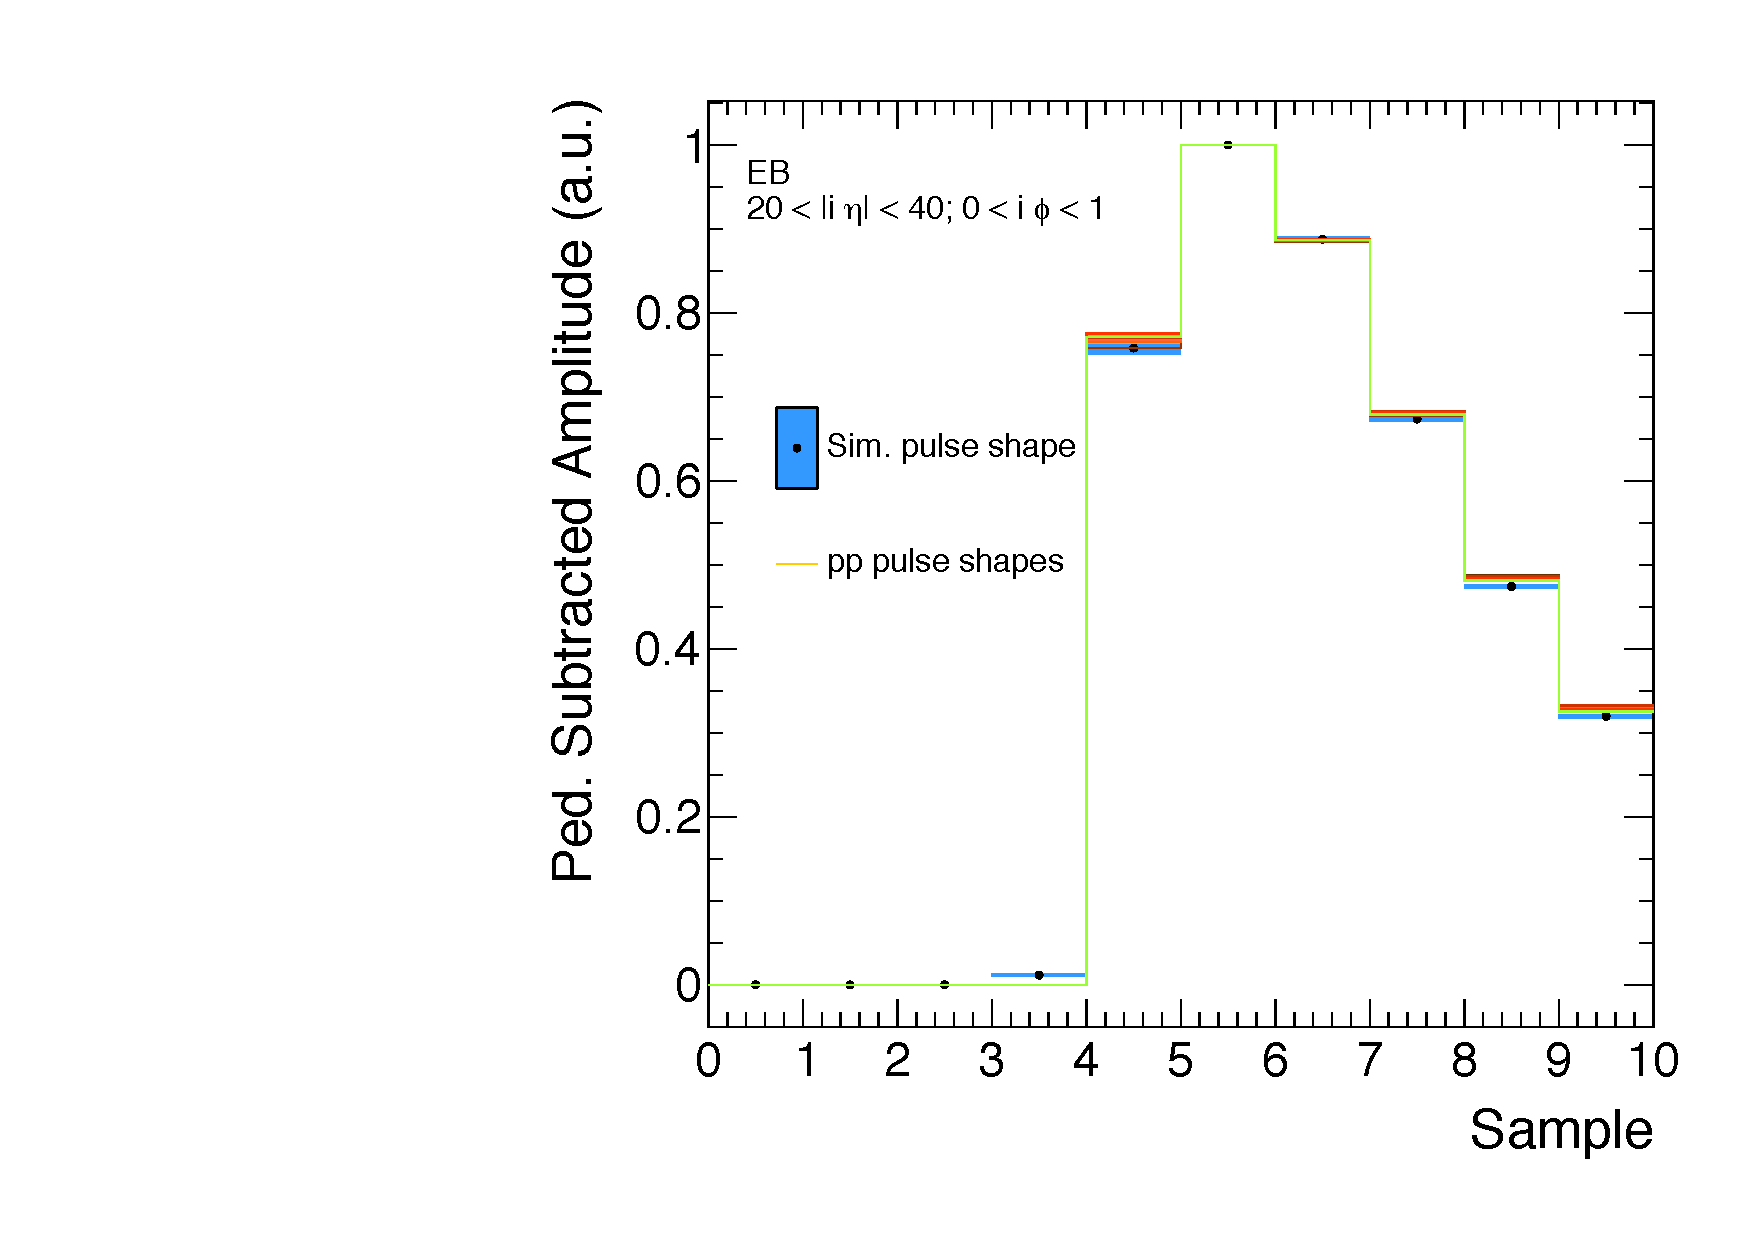
\includegraphics[width=3.0in]{template_EB}\label{fig:pulse_shapes_template}}
%%     \subfigure[]{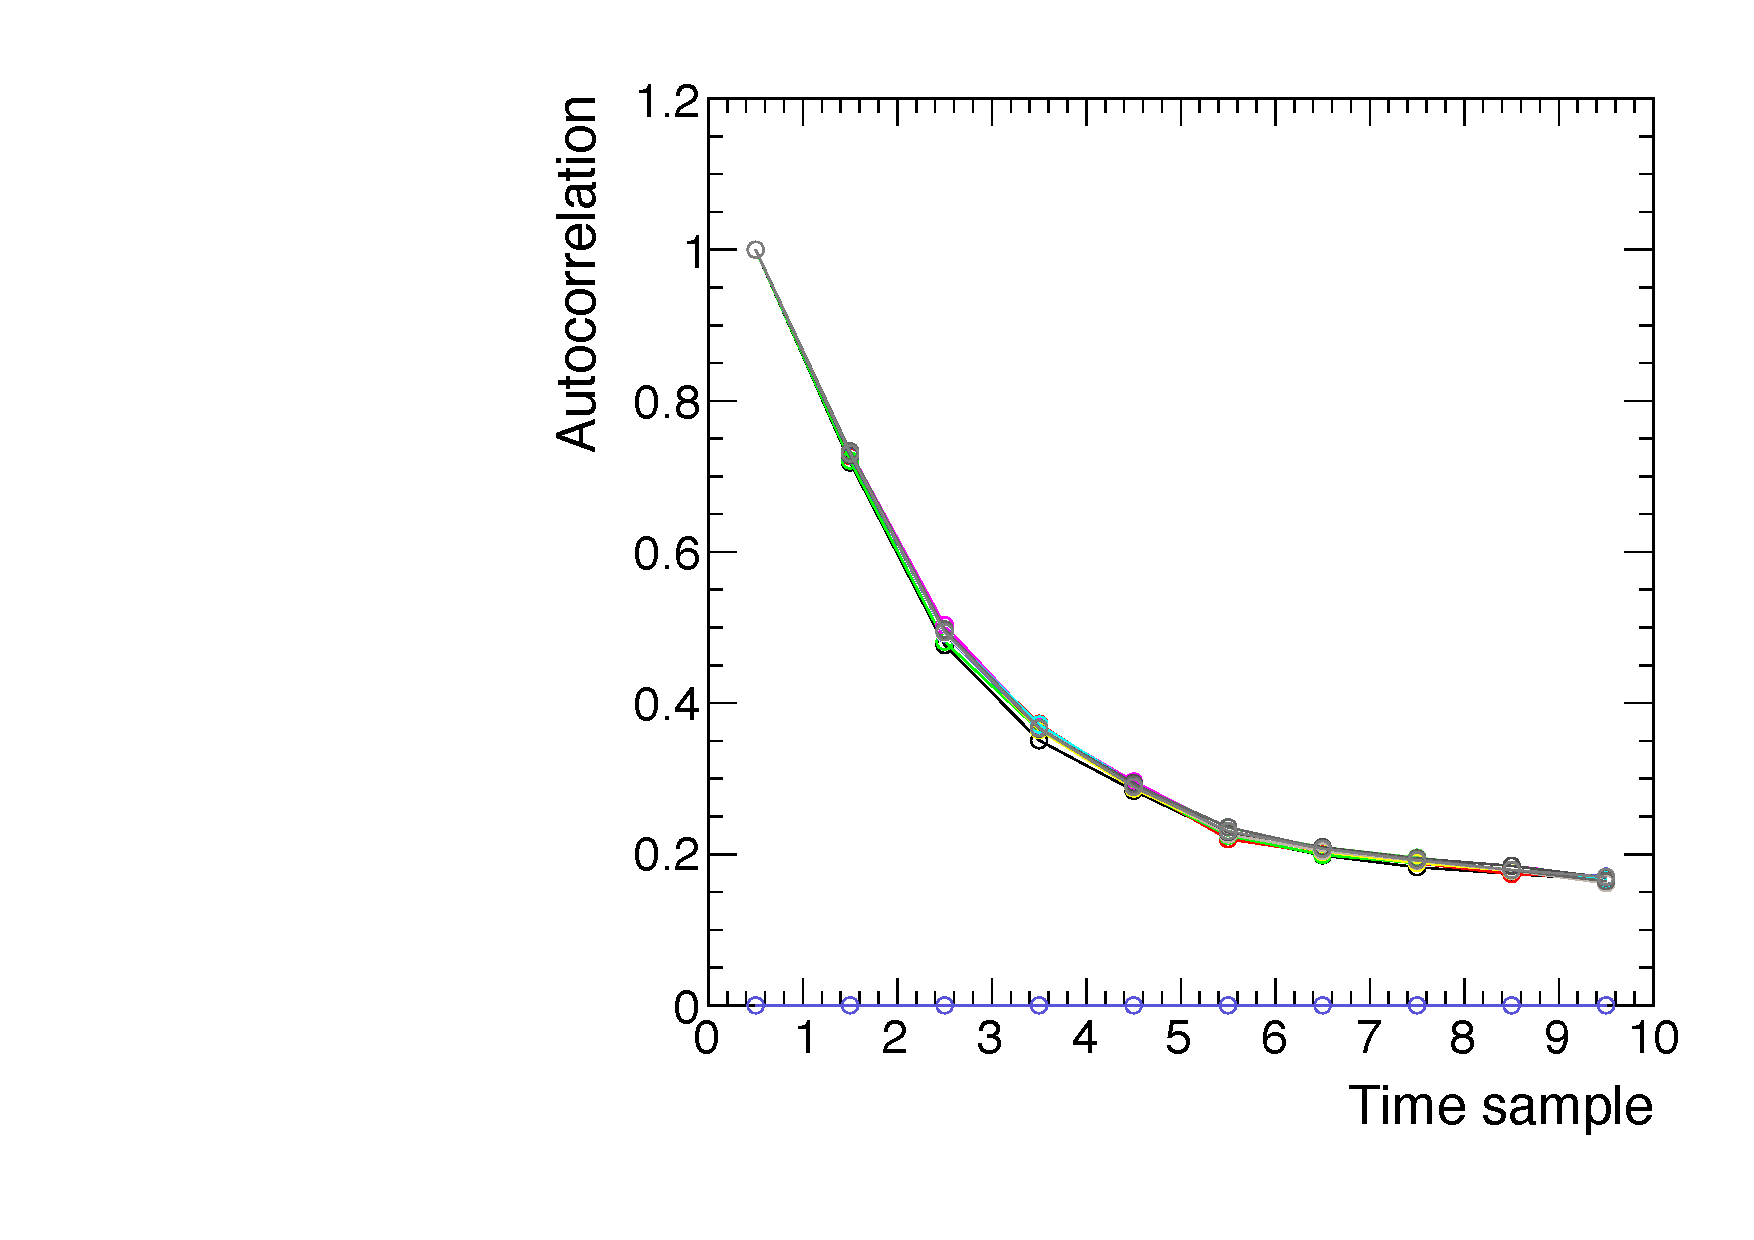
\includegraphics[width=3.0in]{autocorrelation_barrel}\label{fig:noise_autocorrelation}}
%%     \caption{Examples of pulse shapes measured on data in the barrel, after time inter-calibration, compared with the one used in the simulation, averaged over the full barrel, with its uncertainty band (a). Example of the noise autocorrelation measured on 2012 data, for several partitions of the barrel (b). \label{fig:pulse_shapes} }
%%   \end{center}
%% \end{figure}


%Given the number of allowed pulses is $N=10$ for the 25 ns bunch spacing case, in order to have always a constrained fit with the 10 digitized samples we impose that each of the amplitudes is positive. 
The technique of Non-Negative-Least-Squares \cite{nnls} is used to perform the $\chi^2$ minimization of Eqn.~\ref{eqn:chi2multifit} with the constraint that the fitted amplitudes are all positive. Examples of one fit for a hit in the barrel and a hit in the endcap are shown in Fig.~\ref{fig:multifits}. The fit is performed in approx 10 ms/event for events with an average pileup of 40 and for 25 ns bunch spacing.
%
\begin{figure}[!t]
  \begin{center}
    \subfigure[]{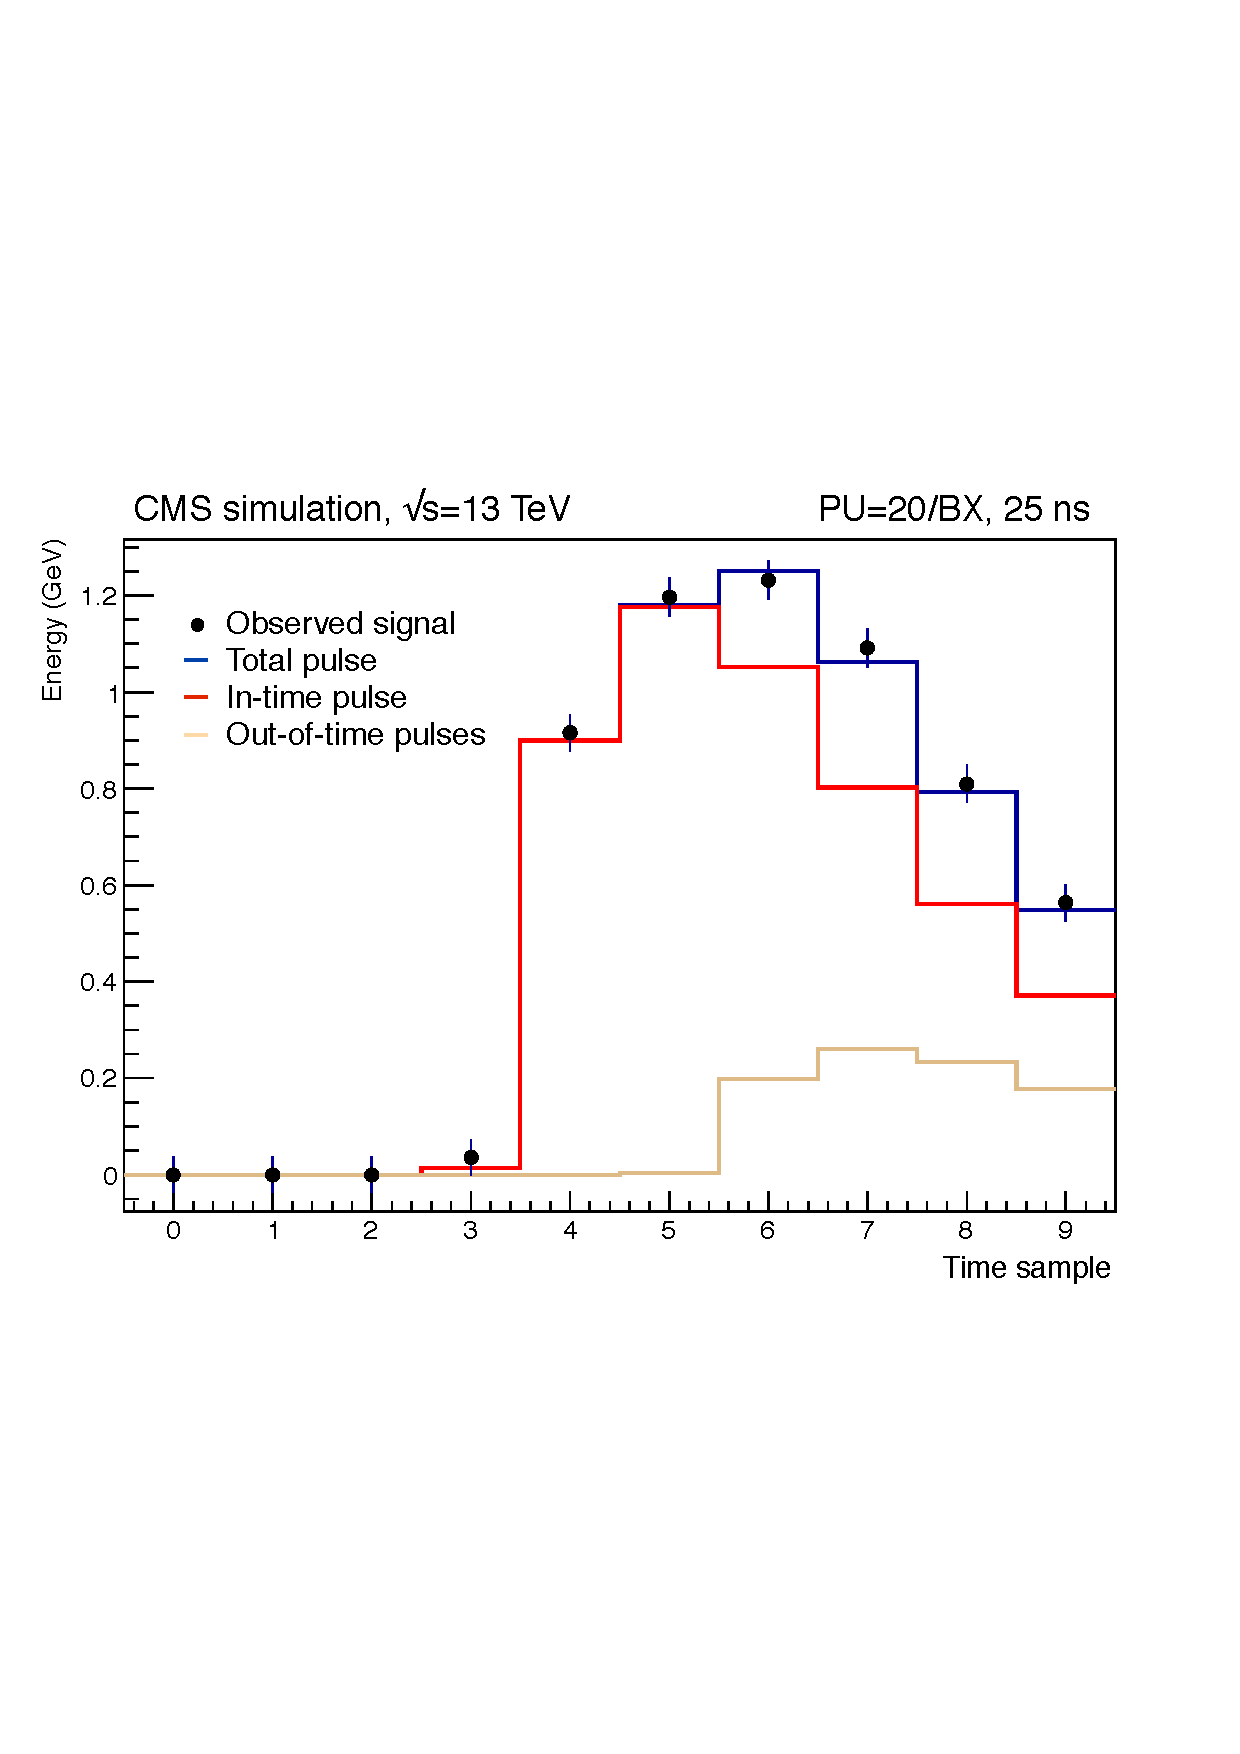
\includegraphics[width=3.1in]{multifit_EB}\label{fig:multifit_EB}}
    \subfigure[]{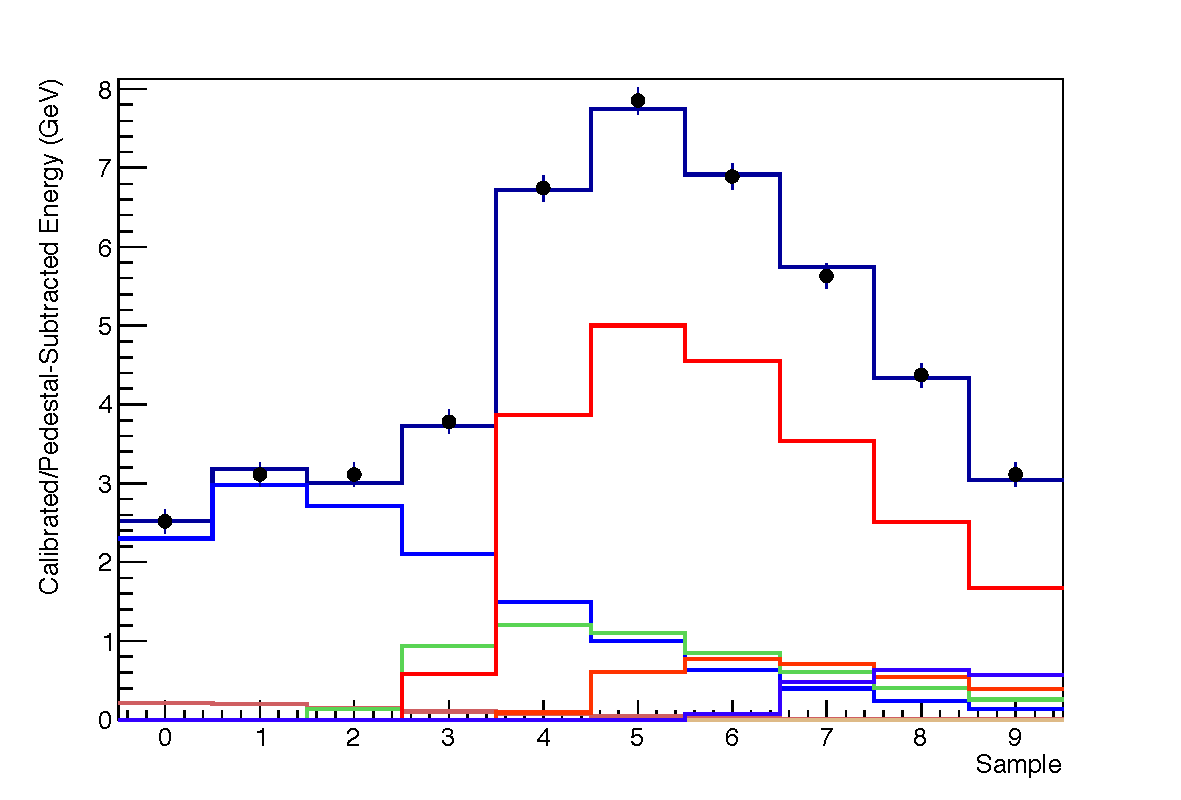
\includegraphics[width=3.1in]{multifit_EE}\label{fig:multifit_EE}}
    \caption{Two examples of fitted pulses for simulated events with 20 average pileup interactions and 25 ns bunch spacing, for a signal in the barrel (a) and in the endcaps (b). Dots represent the 10 digitized samples, the red distributions (other light colors) represent the fitted in-time (out-of time) pulses with positive amplitude. The dark blue histograms represent the sum of all the fitted contributions.  \label{fig:multifits} }
  \end{center}
\end{figure}

The residual contribution of out-of-time pileup to the energy resolution has been estimated for the multi-fit algorithm using simulated samples of unconverted photons. It is observed to be highly suppressed for signal pulses in both the barrel and endcaps. The improvement in energy resolution  with respect the Run I reconstruction algorithm for collisions with 25 ns bunch spacing is substantial especially for low $p_T$ photons and electrons, given the larger contribution of pileup to the total energy estimate, and is still significant for those at high $p_T$ ($p_T>$50 GeV). The new algorithm is thus expected to reduce the pileup dependence in the electromagnetic components of reconstructed jets and $\ETslash$ in Run II.

\subsection{Clustering algorithms}
\label{sec:clustering}
Electrons and photons deposit their energy over several ECAL channels. In addition, the presence of material in front of ECAL causes conversions of photons and bremsstrahlung from electrons, and the radiated energy is spread along $\phi$ by the strong magnetic field. Clustering algorithms are used to collect the energy deposits in ECAL, including the contributions from this radiated energy. For LHC Run II the clustering algorithms will be modified such that the correlation in the $\eta-\phi$ plane of the radiated energy due to the combined effect of the magnetic field and material budget distribution is taken into account. The electron or photon energy is then estimated as:
\begin{equation}
\label{eqn:energy}
E_{e,\gamma} = F_{e,\gamma}\left[G \times \sum_i(C_i \times S_i(t) \times {\cal A}_i + E_{ES}\right]
\end{equation}
where the sum is performed over all the clustered channels. The amplitude measured in the $i$-th channel is labeled by ${\cal A}_i$, while $S_i(t)$ is a time dependent correction that accounts for time variation of the channel response due to changes in crystal transparency. The $C_i$ parameter is a relative calibration constant that takes into account differences in the crystal light yields and photodetector response and $G$ is a scale factor converting the digital scale into GeV. For clusters in the endcap region the corresponding energy in the preshower ($E_{ES}$) is added. Finally $F_{e,\gamma}$ is a particle dependent correction applied to the clustered energy. It accounts for biases in the energy reconstruction related to the geometry of the detector, the upstream material, and the clustering of energy emitted by bremsstrahlung or photon conversions. The pileup dependence of the energy scale and its correlation with the cluster shape and position is taken into account by a multivariate algorithm trained on simulated samples of electrons and photons.  Residual data/simulation differences are accounted for by in-situ measurements using copious physics processes producing electrons and photons in the final state: $\pi^0,\eta\to\gamma\gamma$, $W\to e\nu$, $Z\to e^+e^-$.



\section{Energy calibrations}
\label{sec:energycalibration}
\IEEEPARstart{I}{n} the following section the calibration of the ECAL response and the resulting performance on 2012 data are illustrated. The calibration procedures are expected to remain the same during Run II, while reoptimizations of the calibration streams are necessary, to cope with the increased rates and larger data volumes expected at the HLT. For a detailed description of the ECAL calibration procedures the reader is referred to~\cite{Chatrchyan:2013dga}.

\subsection{Corrections for time-dependent response changes}
\label{sec:timedependence}
Ionizing radiation creates color centers in the crystals reducing their transparency and therefore reducing their measured response to the deposited energy. The color centers partially anneal with thermal energy such that the loss in transparency depends on the dose rate, which varies with $\eta$, and a partial recovery of transparency is observed in the absence of radiation. The changes in transparency are measured and corrected using a dedicated ``laser monitoring'' system \cite{Anfreville:2007zz} which injects laser light ($\lambda \sim 440$ nm, close to the peak of the scintillation light spectrum for $\rm PbWO_4$) into each crystal. One measurement point per crystal is typically recorded every 30 minutes. The change in transparency ($R/R_0$) does not directly measure the change in the amount of the scintillation light ($S/S_0$) since the two have different spectra and the optical photons travel different paths to reach the photodetectors, but they can be related by a power law:
\begin{equation}
\label{eqn:alpha}
\frac{S}{S_0} = \left(\frac{R}{R_0}\right)^\alpha
\end{equation}
where $\alpha ~\sim 1.5$.

By the end of LHC Run I in 2012 the loss in transparency was up to 6\% in EB and up to 30\% in the EE region within the tracker acceptance ($\vert\eta\vert<2.5$), reaching 70\% in the most forward EE regions ($\vert\eta\vert>2.7$). The corrections for transparency loss (LC) were validated with collisions data, by examining the stability of the reconstructed invariant mass of $\pi^0$ decays and and using the ratio of $E/p$ for isolated electrons from $W\to e\nu$ and $Z\to e^+e^-$ decays. In the ratio, $E$ is the energy measured in the calorimeter and $p$ is the momentum measured in the tracker. Figure \ref{fig:EoP_2012} shows the stability of the $E/p$ ratio measured from 2012 data before and after the LC are applied. The stability of the ratio after corrections is better than 0.1\% in the barrel and 0.4\% in the endcaps.  Any residual imperfections in the LC (e.g. due to the dispersion in $\alpha$ values between crystals) are removed by applying additional time-dependent corrections, explained below.
%
\begin{figure}[!t]
  \begin{center}
    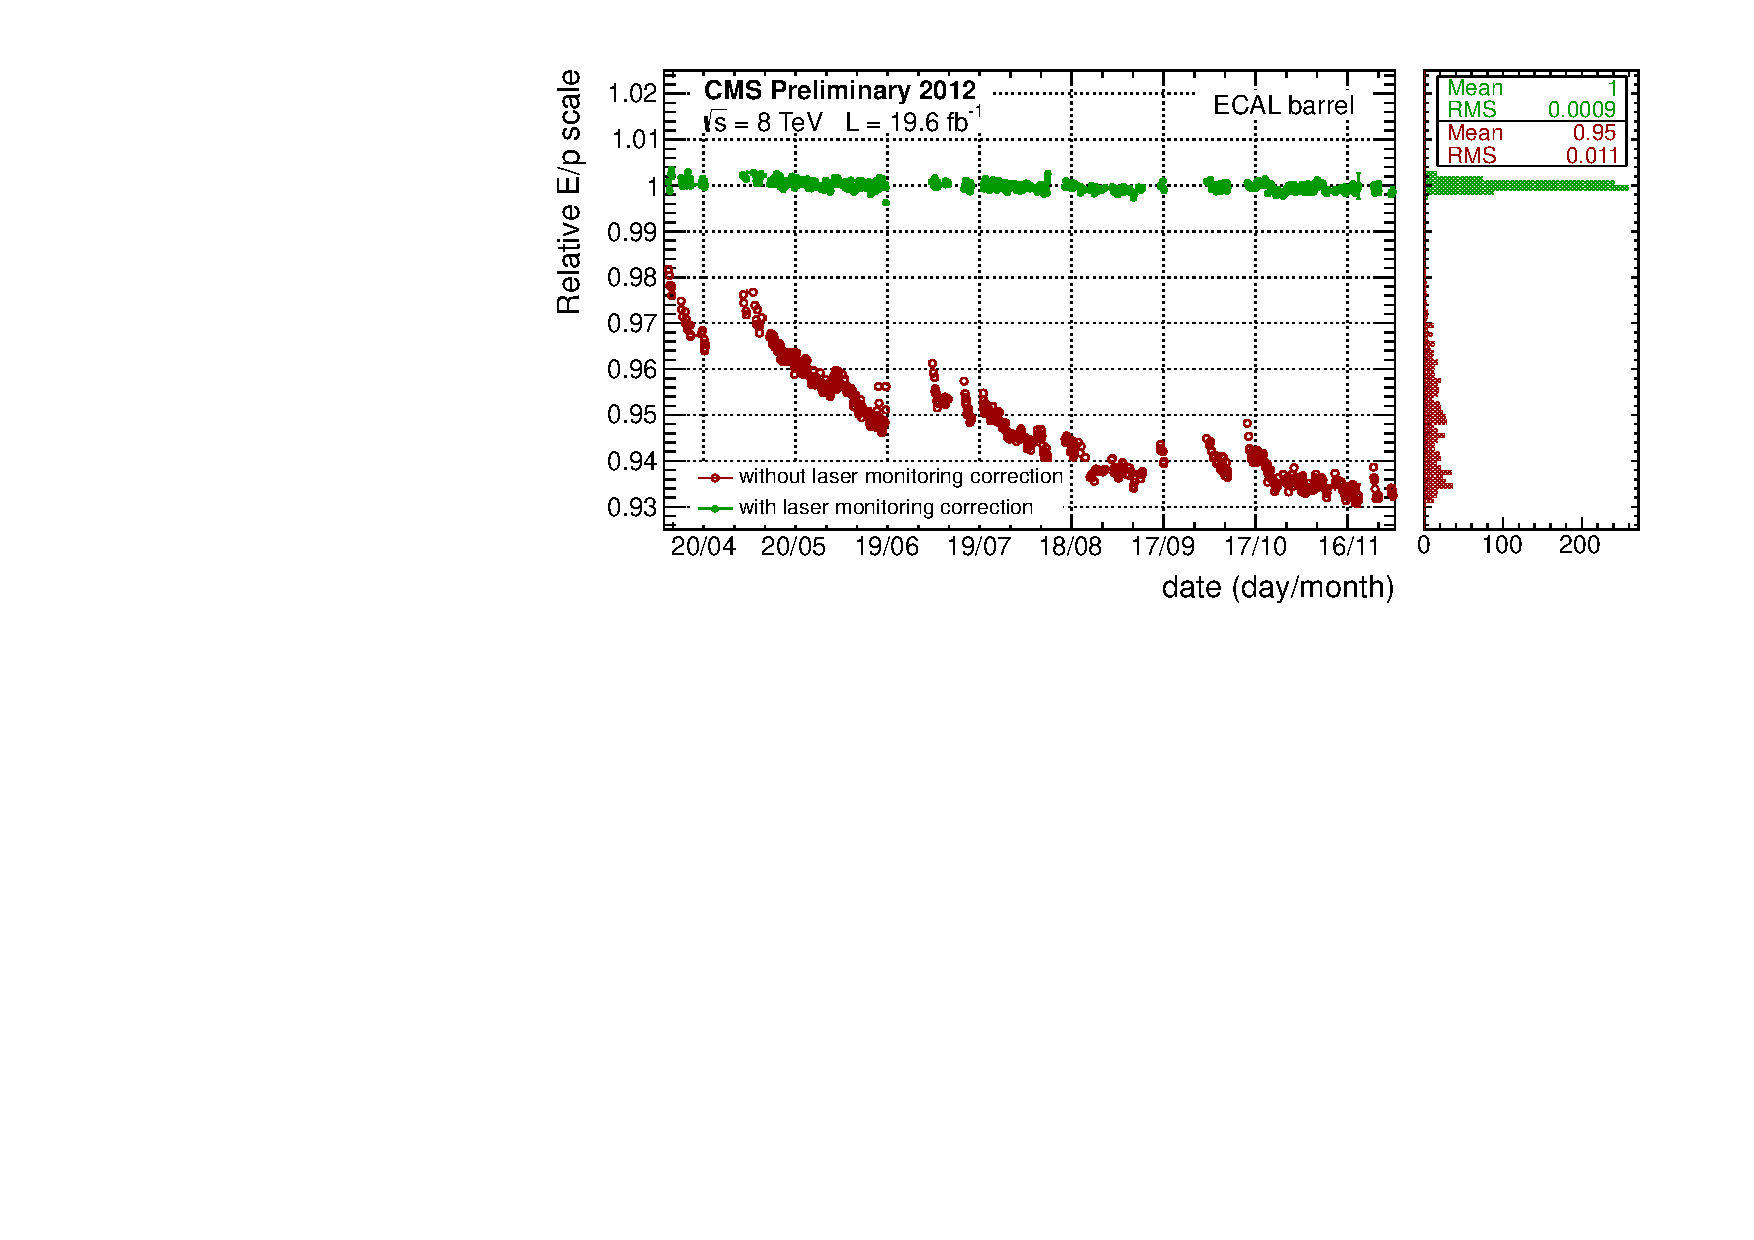
\includegraphics[width=3.5in]{EoP_EB_Winter2013}
    \caption{History plot for 2012 data of the ratio of electron energy E, measured in the ECAL Barrel, to the electron momentum p, measured in the tracker.  The electrons are selected from $W\to e\nu$ decays. The projections along the Y axis are shown in the histograms on the right side. \label{fig:EoP_2012}}
  \end{center}
\end{figure}


For Run II one of the main challenges is to maximise the number of $W\to e\nu$ decays available for calibration purposes give the limited bandwidth available to single electron triggers in 2015. A dedicated HLT stream has thus been developed that reduces the output bandwith per event by saving only the hits of the tracker and ECAL partitions traversed by the reconstructed electron. In addition, several global event variables are saved in this stream to define the event selection and the cluster corrections, such as the $\ETslash$, the average energy density of the event, and the HCAL over ECAL cluster energy ($H/E$) ratio. 
Event displays of a $W\to e \nu$ interaction with the standard reconstruction and with the reduced event content for the calibration HLT stream are shown in Fig.~\ref{fig:elestream_before} and \ref{fig:elestream_after} respectively. The event size is typically reduced by a factor of 5 to 10.
%
\begin{figure}[!t]
  \begin{center}
    \subfigure[]{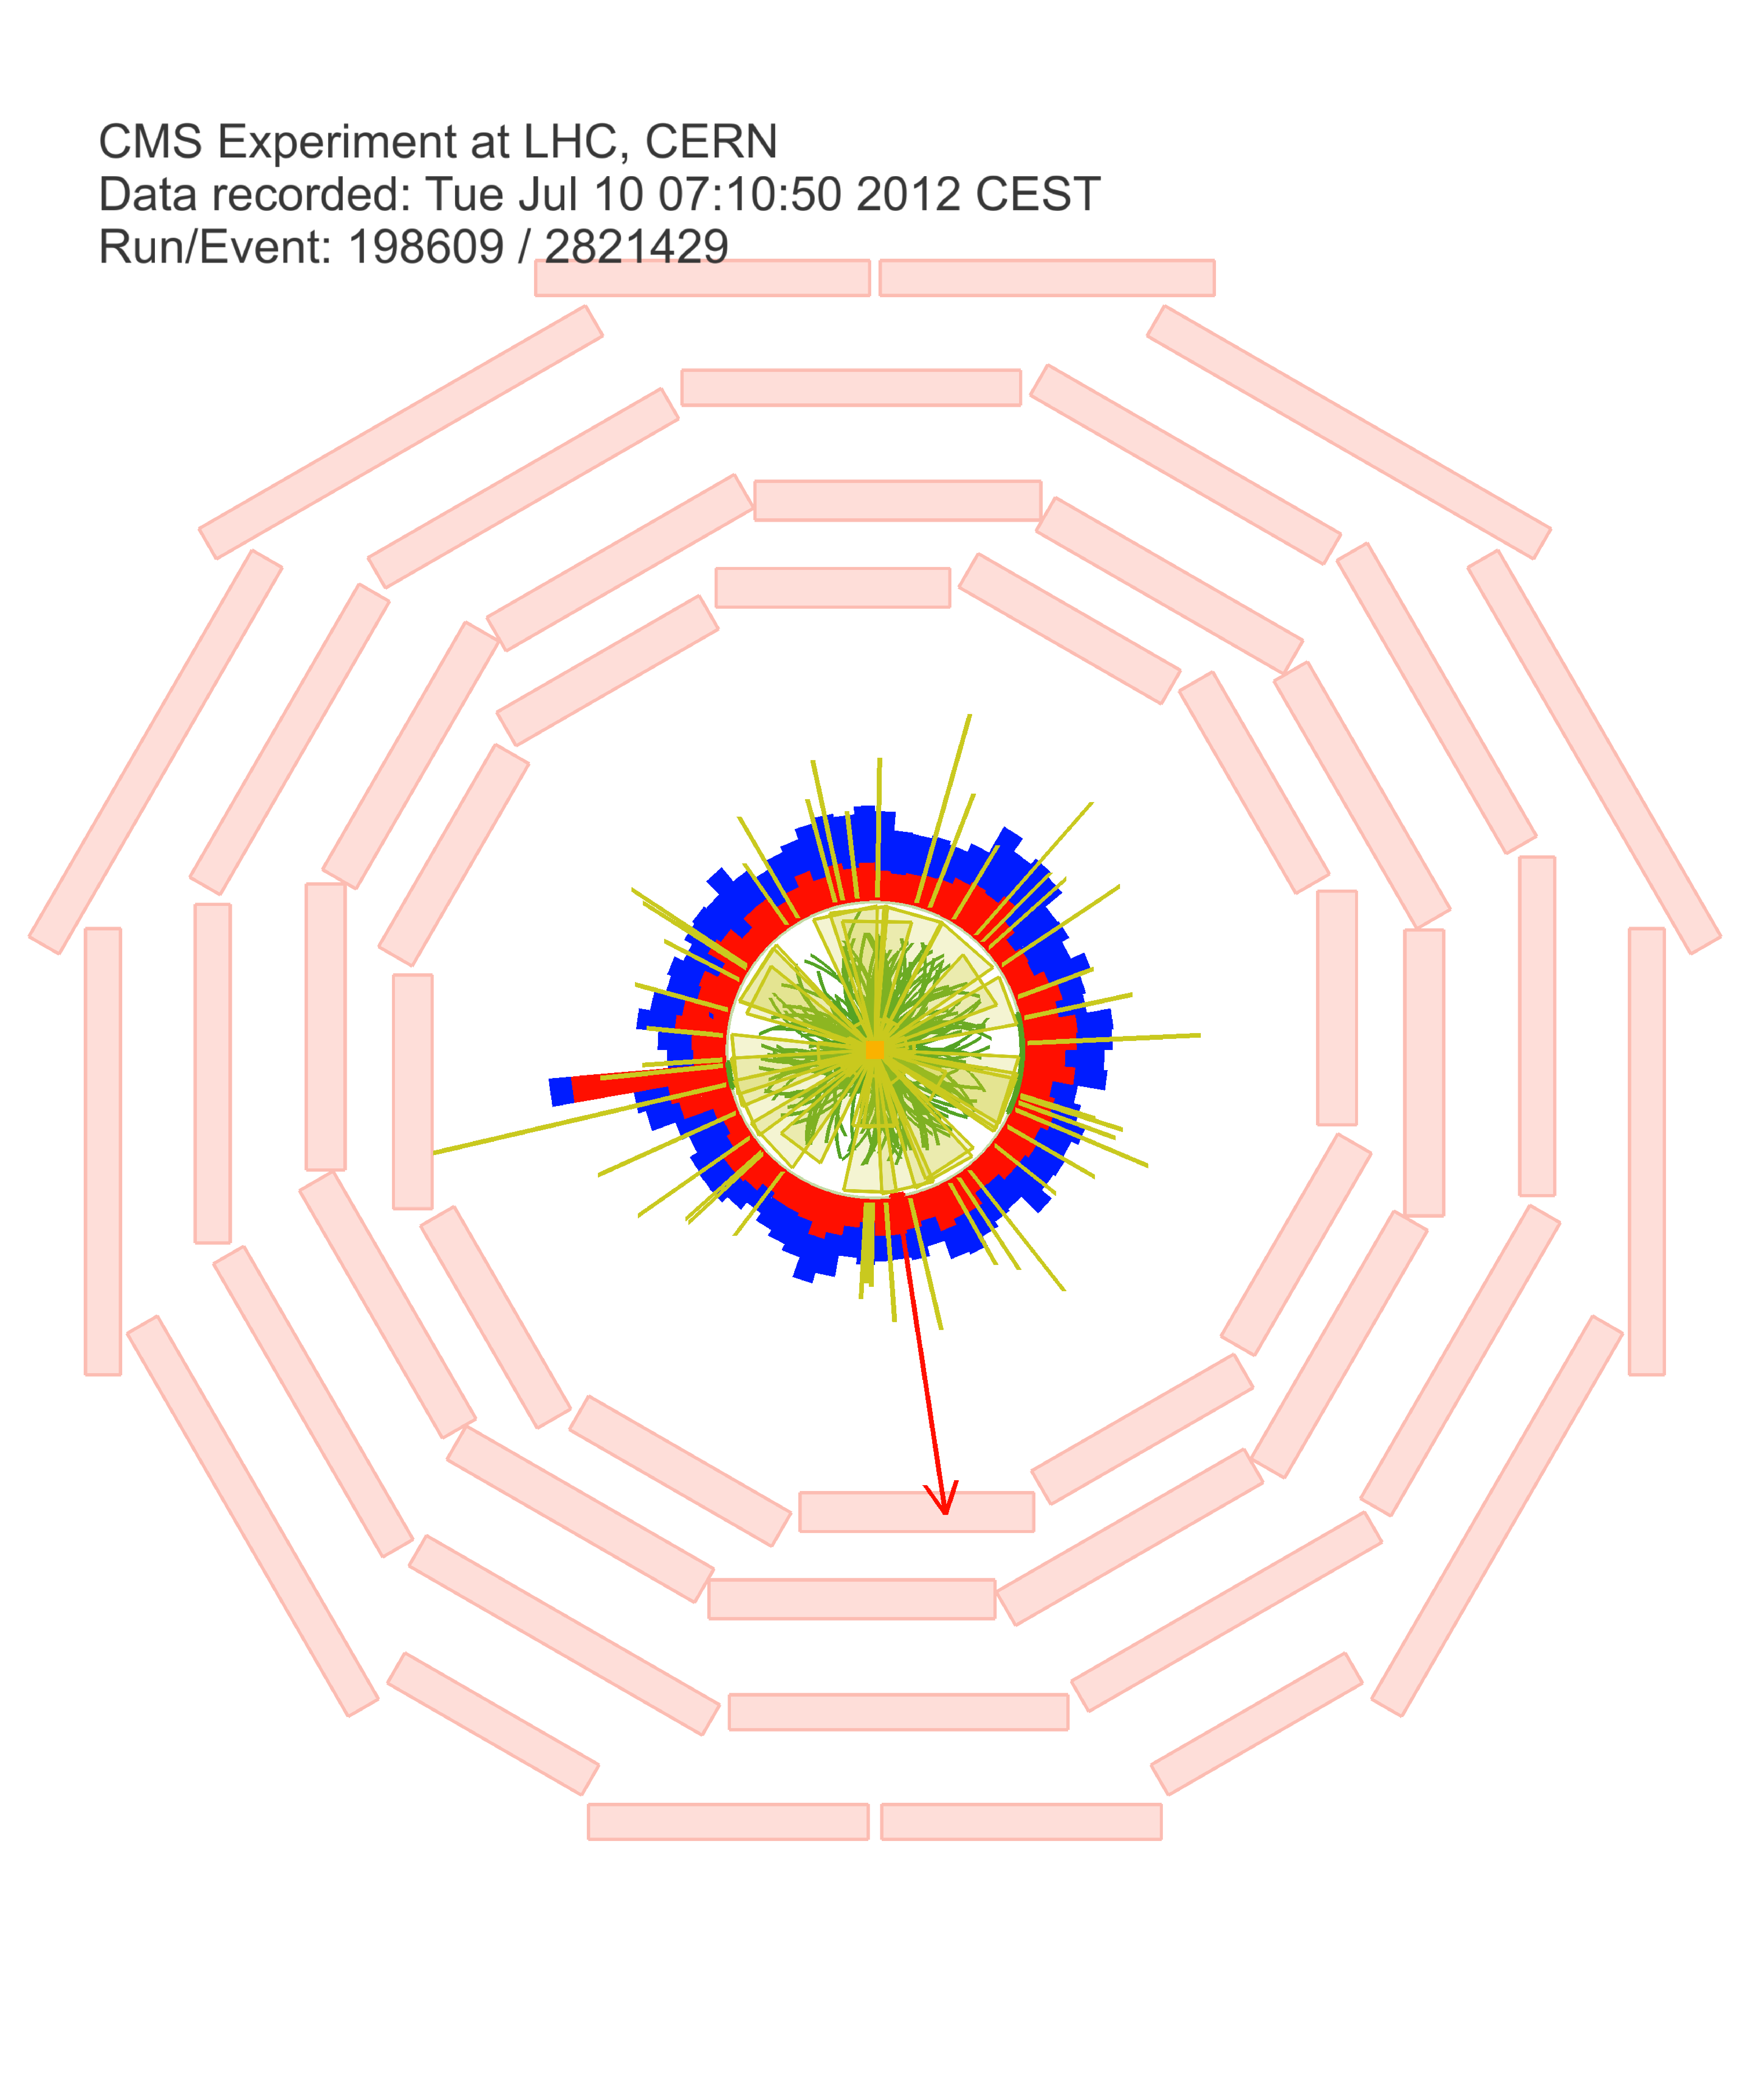
\includegraphics[width=1.6in]{wenu_reco}\label{fig:elestream_before}}
    \subfigure[]{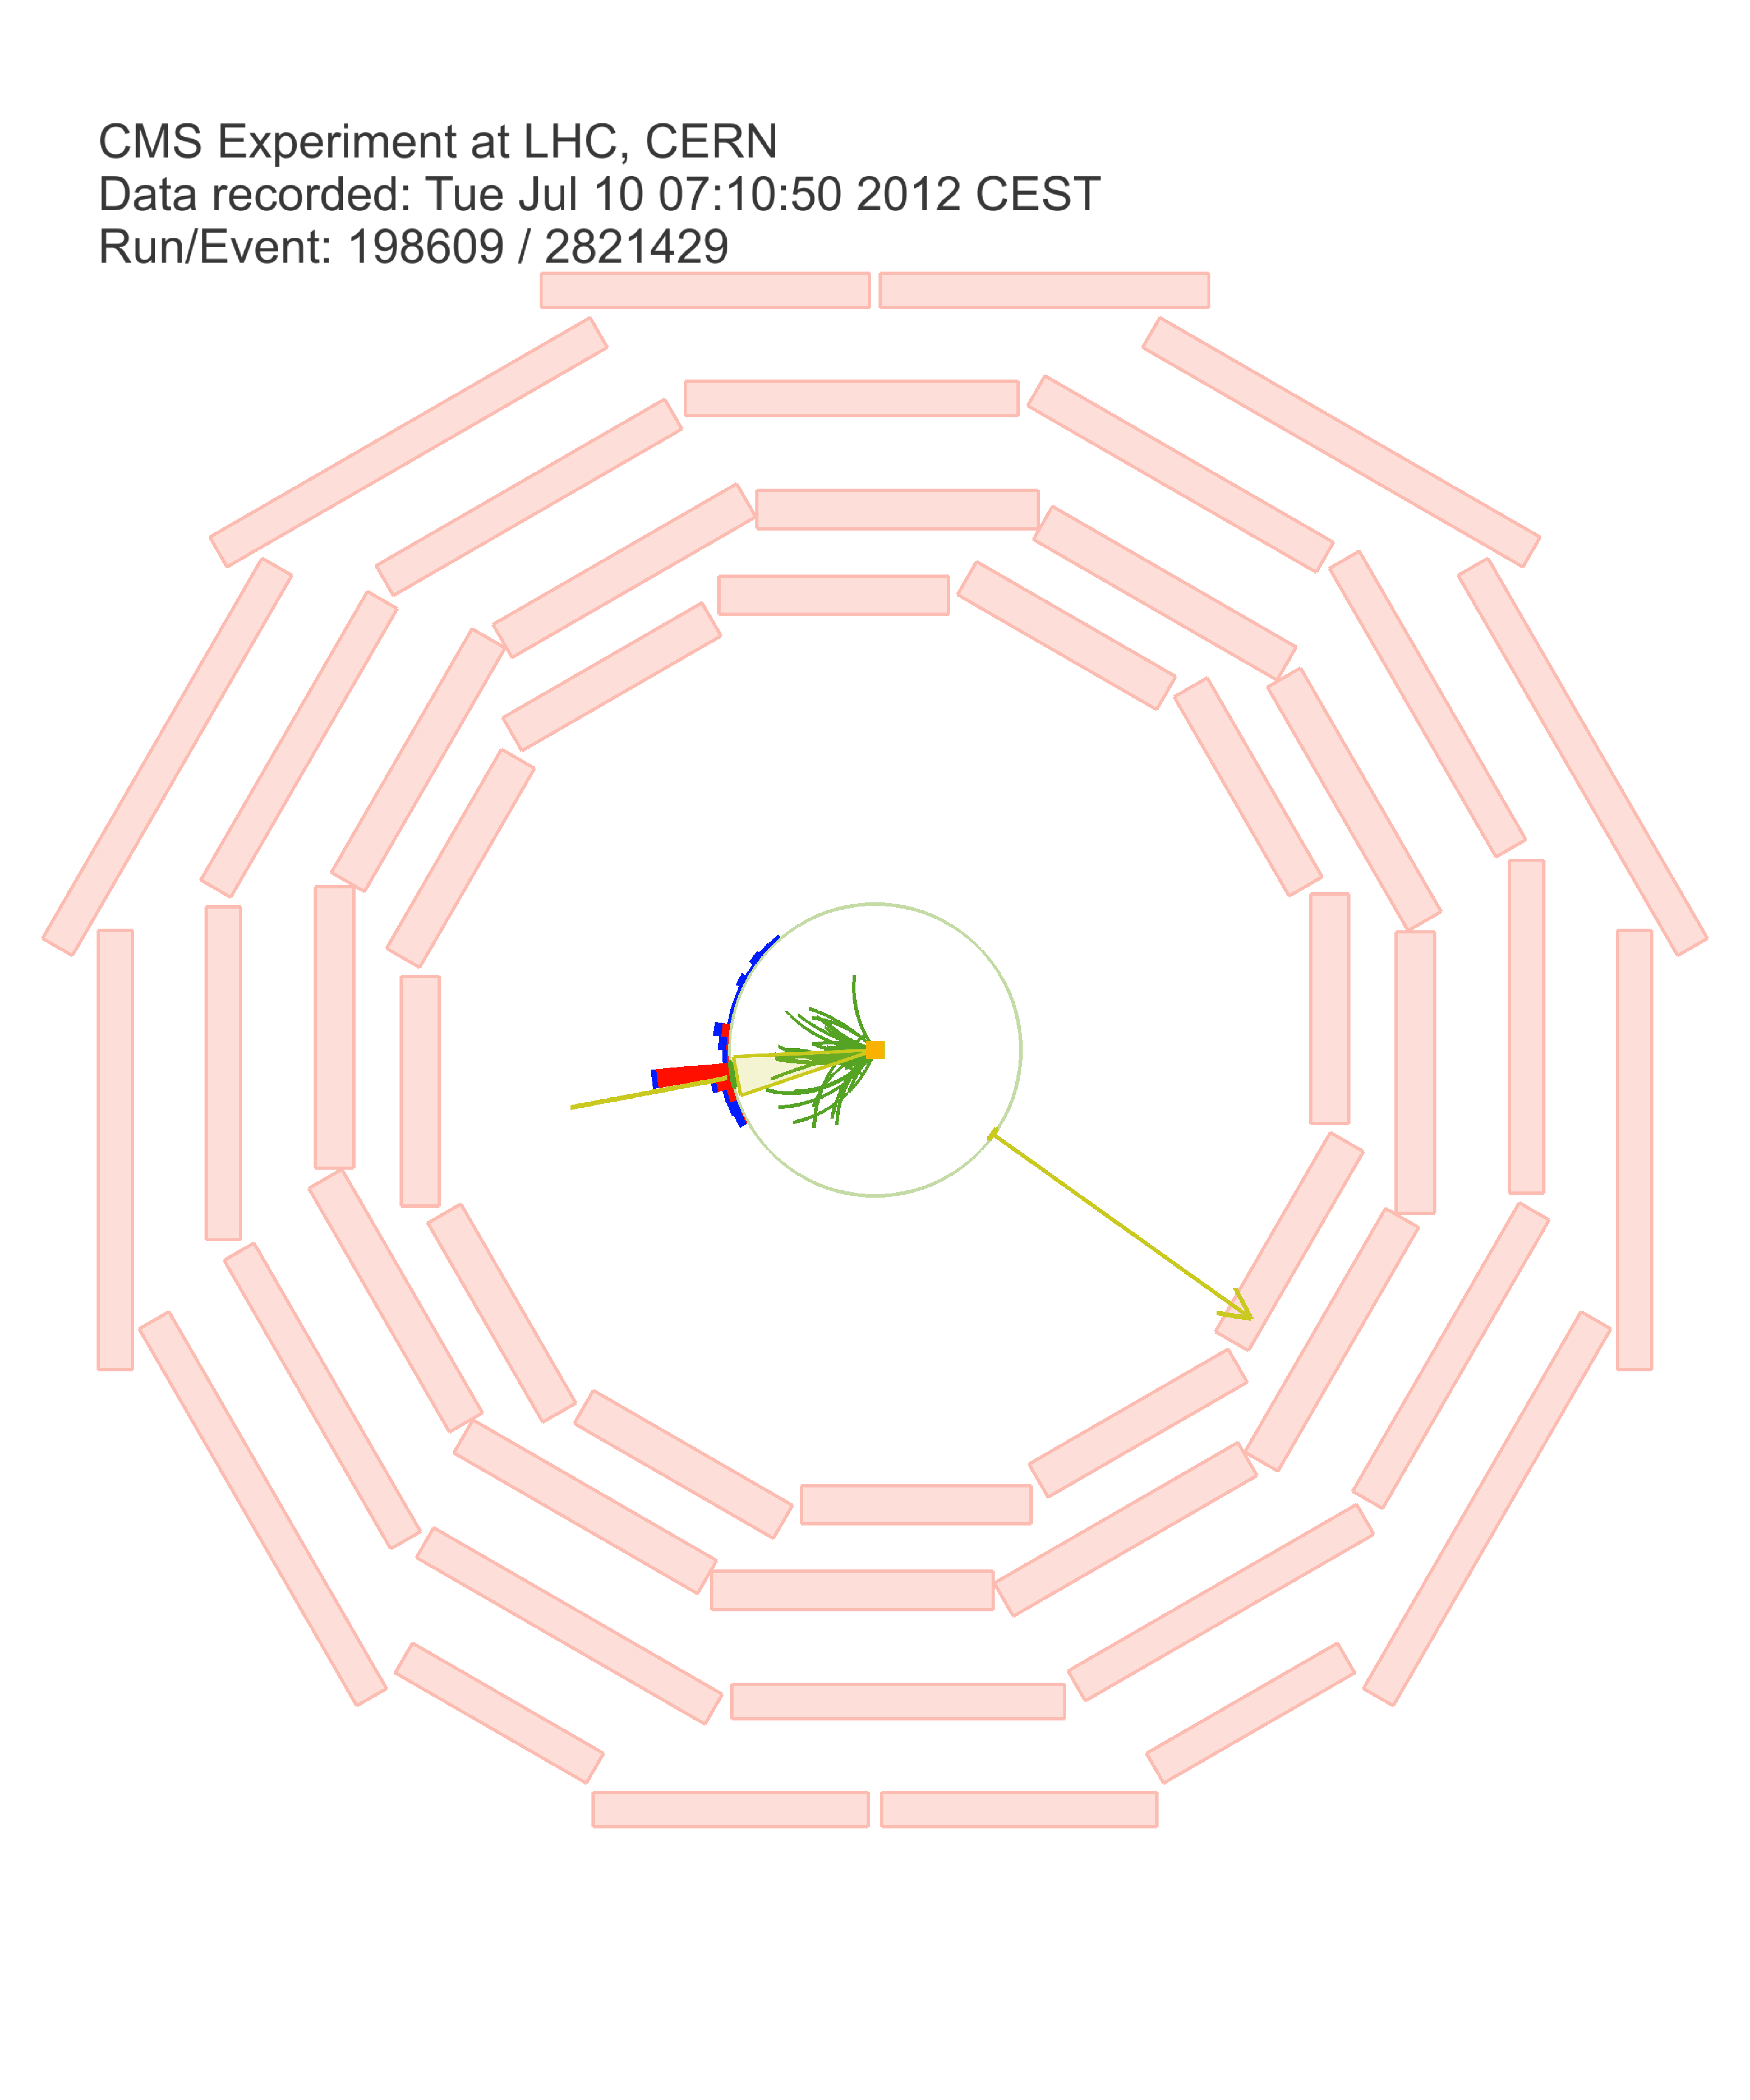
\includegraphics[width=1.6in]{wenu_stream}\label{fig:elestream_after}}
    \caption{Event displays of a $W\to e\nu$ event reconstructed offline, with the full event content (a) and after the event content has been stripped to save only the hits around the electron (a). On Fig. (a), the red arrow shows the reconstructed $\ETslash$, on Fig. (b), the yellow arrow shows the $\ETslash$ as estimated from the HLT reconstruction. \label{fig:elestream}}
  \end{center}
\end{figure}
%


\subsection{Intercalibrations and energy scale}
\label{sec:intercalibrations}
Relative calibration of the crystals (parameter $C_i$ in Eqn.~\ref{eqn:energy}) is obtained from LHC collisions data. These intercalibration constants (IC) are calculated using several independent methods, and the resulting constants are combined to provide one number per crystal. These methods include the use of azimuthal symmetry of the energy flow in minimum bias events (``$\phi$ symmetry''), the invariant mass of photon pairs from $\pi^0$ and $\eta$ decays, and the $E/p$ ratio of isolated electrons from $W\to e\nu$ and $Z\to e^+e^-$ decays.

The $\phi$-symmetry method is based on the equalization of the average energy measured in different channels located at a constant value of $\eta$. It employs a dedicated data stream with reduced event information. The stream records a high rate of events ($\sim$1.5 kHz) and the method achieves a statistical precision of better than 0.2\% (0.4\%) in EB (EE) for a typical LHC fill. The accuracy of the method is limited to few percent by systematic uncertainties in the distribution of material in front of the ECAL. Since this uncertainty does not vary with time, the method can be used to track possible time variations in the IC values. In 2012 a drift of the ICs was observed compatible with uncertainties in the LC due to the spread of the value of $\alpha$ in Eqn.~\ref{eqn:alpha}. Corrections that account for these variations are propagated to the final calibration, in time intervals of approximately one month. For 2015 a reoptimization of the thresholds is foreseen in order to cope with the different signal / noise ratio. This stream is not expected to be degraded by the higher pileup, since a larger number of interactions per BX corresponds to a higher rate of minimum bias events available for this calibration method.

The $\pi^0$ mass method is based on the reconstruction of the peak in the spectrum of the invariant mass of unconverted photon pairs from $\pi^0$ and $\eta$ decays. The photons are reconstructed using the energy sum in a $3 \times 3$ matrix of crystals centred on the crystal with the highest energy deposit, and an iterative method is used to determine the IC value of each channel. It employs a dedicated data stream with high rate( $\sim$ 7 kHz) and reaches a precision of 0.5\% in the central barrel ($\vert\eta\vert<0.8$). This precision is dominated by systematic uncertainties. In 2015 with the higher pileup foreseen, the use of the pileup subtracted local reconstruction together with a retuning of the $\pi^0 / \eta$ selections as a function of $\eta$ are expected to maintain the same precision in the central barrel region and improve it in regions that were statistically limited in 2012 (e.g. in the region $\vert\eta\vert\ge2$ where only $\eta$ decays were used). Moreover, the use of particle-flow clusters \cite{CMS:2010eua} will be exploited to benefit from the better cluster calibrations and identification capabilities possible in the HLT.

The $E/p$ method is based on the comparison of the energy measured in the ECAL (Eqn.~\ref{eqn:energy}) to the momentum measured by the tracker for isolated electrons, and an iterative procedure is used to extract the IC value for each channel. The method uses the full 2012 dataset and the precision in the central barrel reaches the systematic limit of 0.5\%, while for $\vert\eta\vert>1$ the statistical contribution is the limiting factor.

The combined intercalibration was obtained from the mean of the individual intercalibration constants at a fixed value of eta, weighted by their respective precisions. In the region $\vert\eta\vert>2.5$, beyond the tracker acceptance, the $E/p$ method can not be used and the high pileup prevents the reconstruction of the invariant mass peak from $\pi^0$ or $\eta$, therefore only the ICs from the $\phi$-symmetry are available. The precision of the different methods and of their combination is reported in Fig.~\ref{fig:intercalib}: it is $\sim$0.3\% ($\sim$0.7\%) in the central (outer) barrel, and $\sim$1.5\% in the endcaps.
%
\begin{figure}[!t]
  \begin{center}
    \subfigure[]{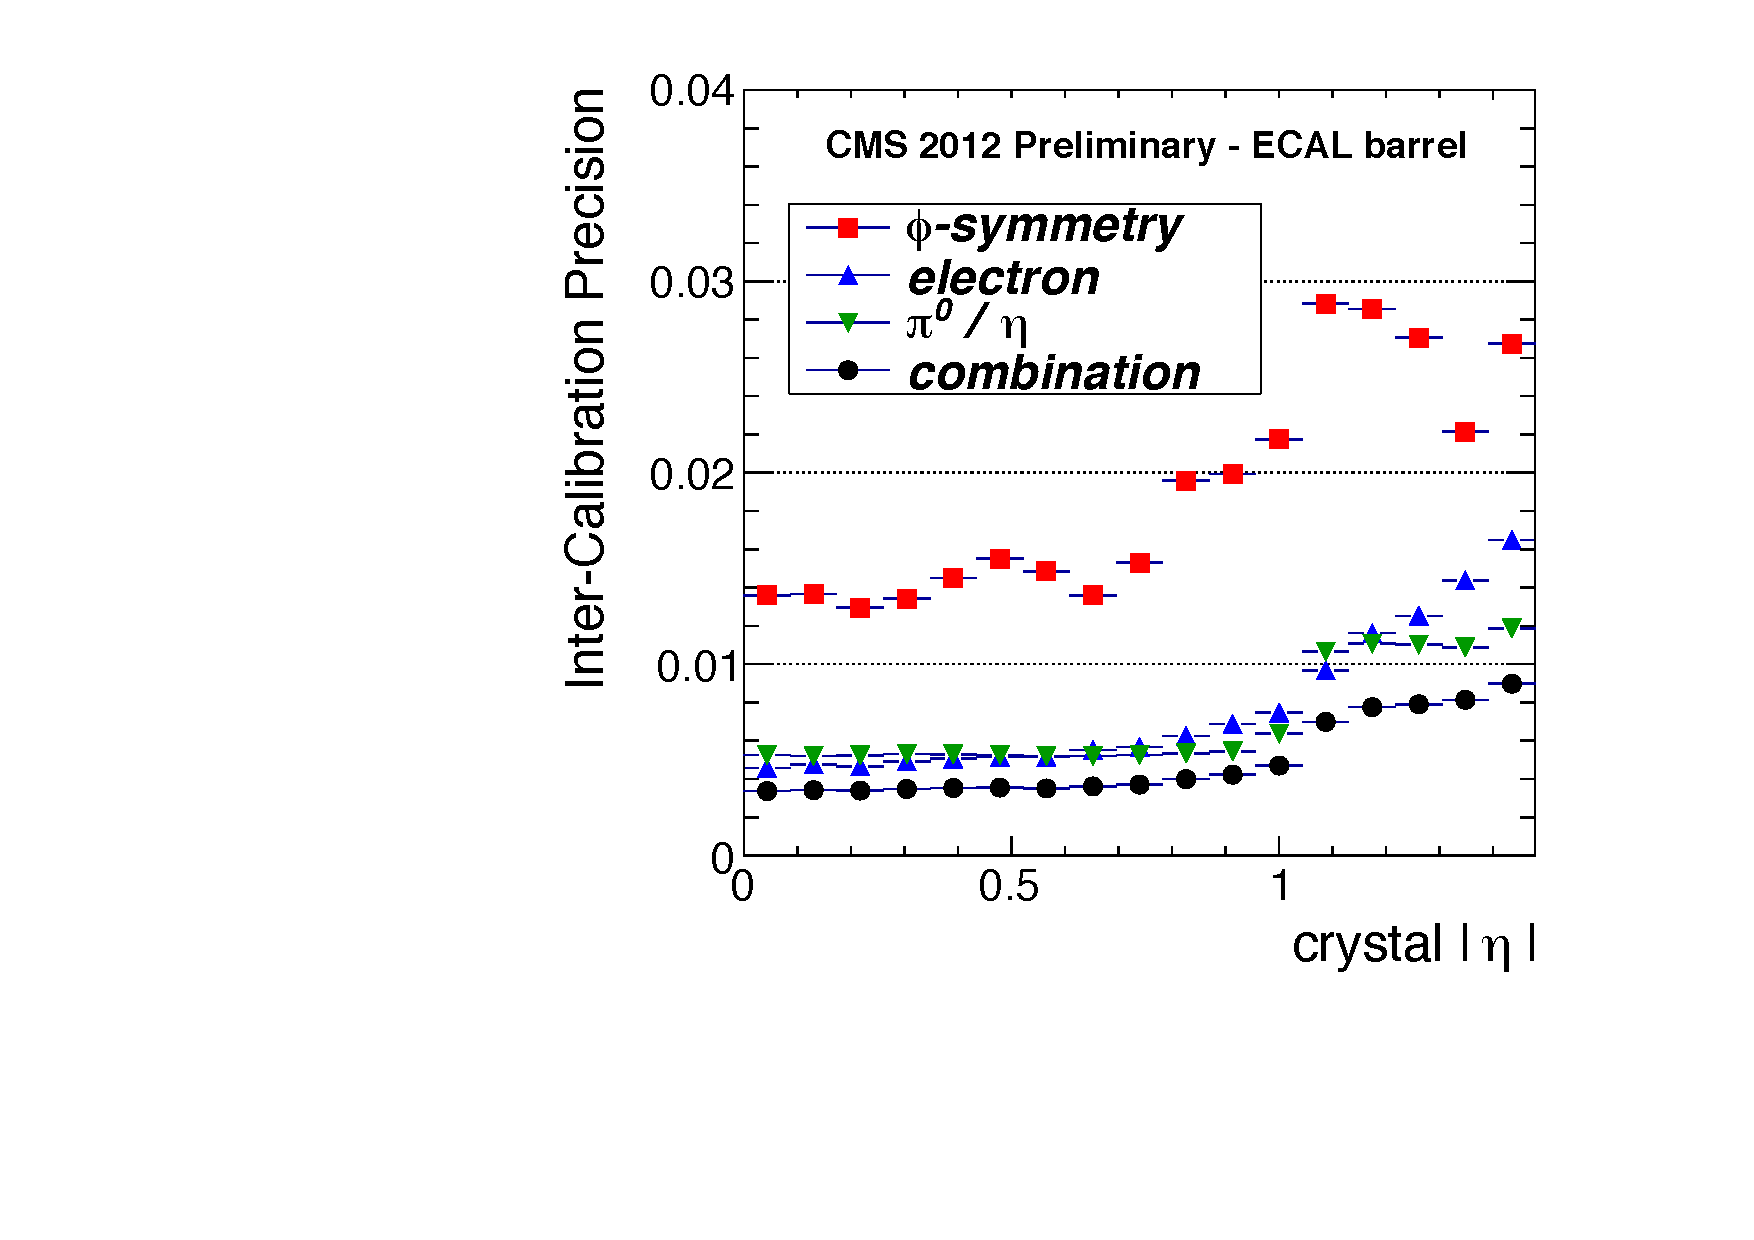
\includegraphics[width=3.0in]{2012EBprecWithCombV3}\label{fig:intercalib_EB}}
    \subfigure[]{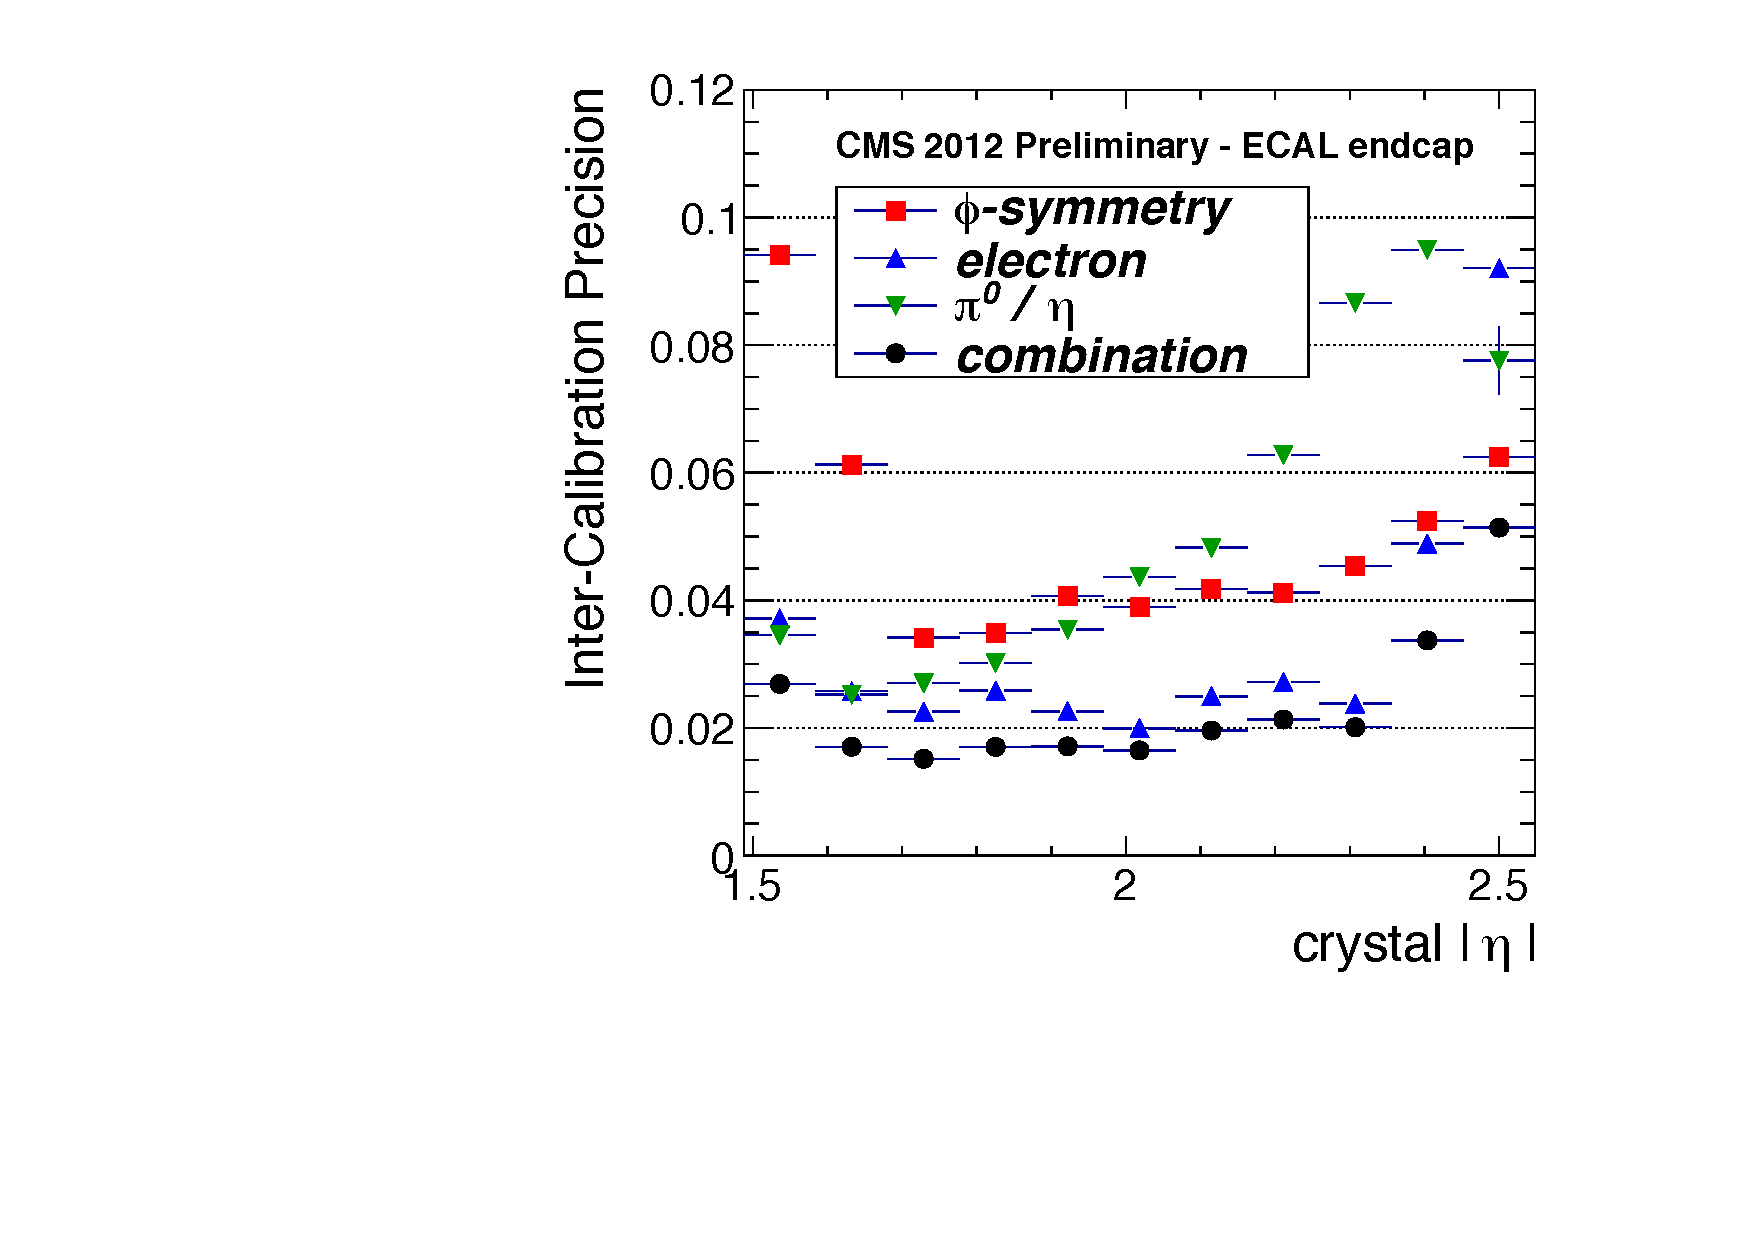
\includegraphics[width=3.0in]{2012EEprecWithCombV3}\label{fig:intercalib_EE}}
    \caption{Precision of the calibration coefficients as a function of $\vert\eta\vert$, for the barrel (a) and the endcaps (b). The precisions of the different methods and of their combination are reported. \label{fig:intercalib}}
  \end{center}
\end{figure}
%

The relative calibration of the $\eta$ rings ($\eta$ scale) is obtained from the invariant mass of $Z\to e^+e^-$ decays, selecting a sample of non-showering electrons. The $\eta$ scale is set to match the expectation from Monte Carlo simulations. The overall energy scale $G$ is set, separately for EB and EE, such that the reconstructed Z peak in data matches that in the Monte Carlo.

For LHC Run II the $Z\to e^+e^-$ decays will be also exploited to provide per-crystal intercalibration constants by employing an invariant mass constraint on the di-electrons. Preliminary studies indicates that this can improve the accuracy of the calibration in the endcap region covered by the tracker. It can also be extended to the region above $\vert\eta\vert=2.5$ by reconstructing one of the two electrons using only calorimetric information. 



\section{Energy resolution and scale}
\IEEEPARstart{T}{he} energy resolution for electrons and photons plays a crucial role in the search for the Higgs boson with electromagnetic final states, and in particular for the search in the Higgs decays channel H$\to\gamma\gamma$. The accuracy of the calibration directly contributes to the energy resolution with a dilution factor of 0.7 due to the sharing of the energy between different channels. 

Figure~\ref{fig:energy_resol_std} shows the measured energy resolution for electrons from $Z\to e^+e^-$ decays plotted as a function of $\vert\eta\vert$ for 2012 data. The resolution is affected by the amount of material in front of ECAL (which increases beyond $\vert\eta\vert>1$) and the presence of cracks between modules (vertical lines in the plot). The resolution is shown for two sets of intercalibration constants: initial calibration constants derived from early 2012 data (grey points) and with calibration constants derived from all 2012 data (blue points). The resolution improves significantly when the full 2012 dataset is used, especially in the endcaps. This indicates that regular calibration is needed to optimise the energy resolution of ECAL, and this will also be required in Run II.

Figure~\ref{fig:energy_resol_std} also shows the resolution expected from Monte Carlo simulations (red points). The residual discrepancy between data and Monte Carlo is accounted for by adding in quadrature a constant Gaussian smearing to the electron and photon energies in Monte Carlo events. Figure~\ref{fig:energy_resol_smeared} shows a comparison of the energy resolution of 2012 data with the tuned simulation.

%
\begin{figure}[!t]
  \begin{center}
    \subfigure[]{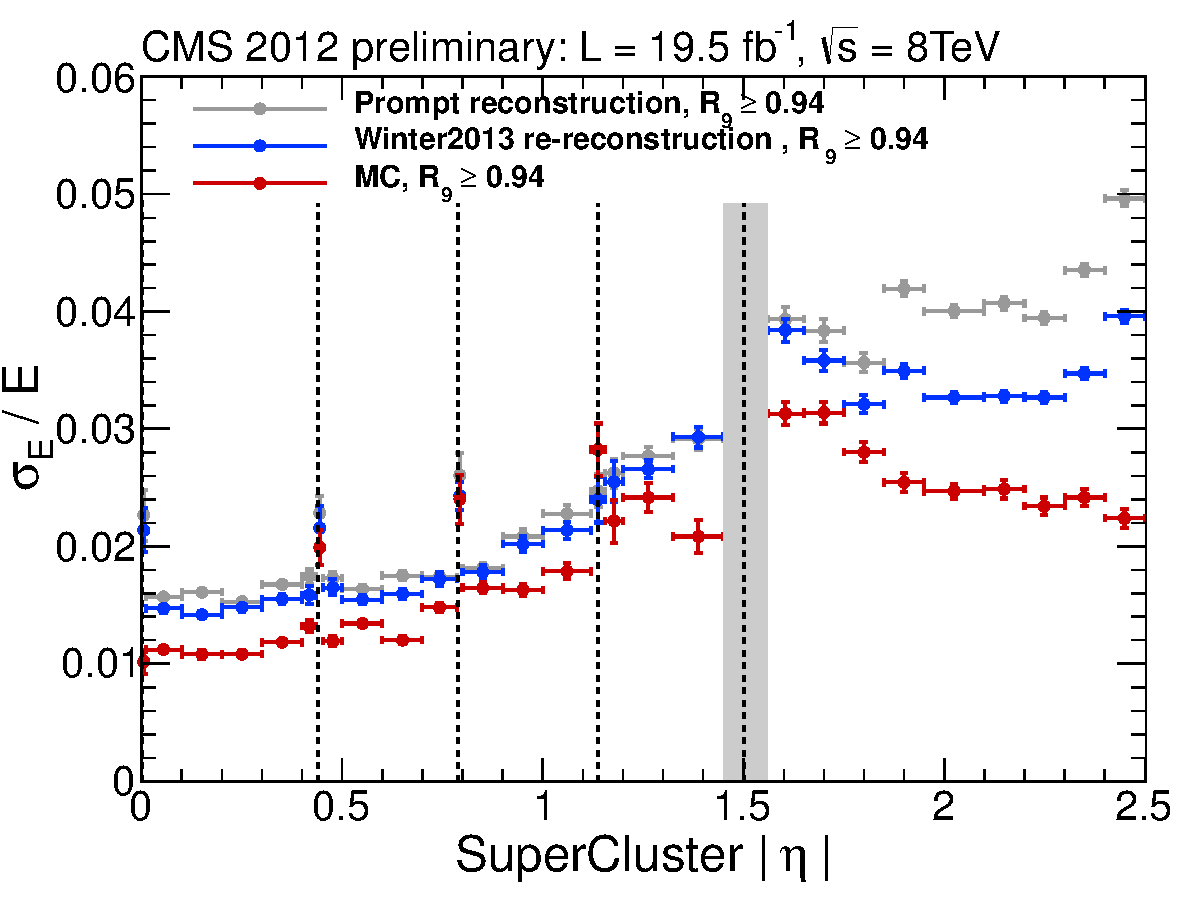
\includegraphics[width=3.0in]{resolution_highR9_beforesmear}\label{fig:energy_resol_std}}
    \subfigure[]{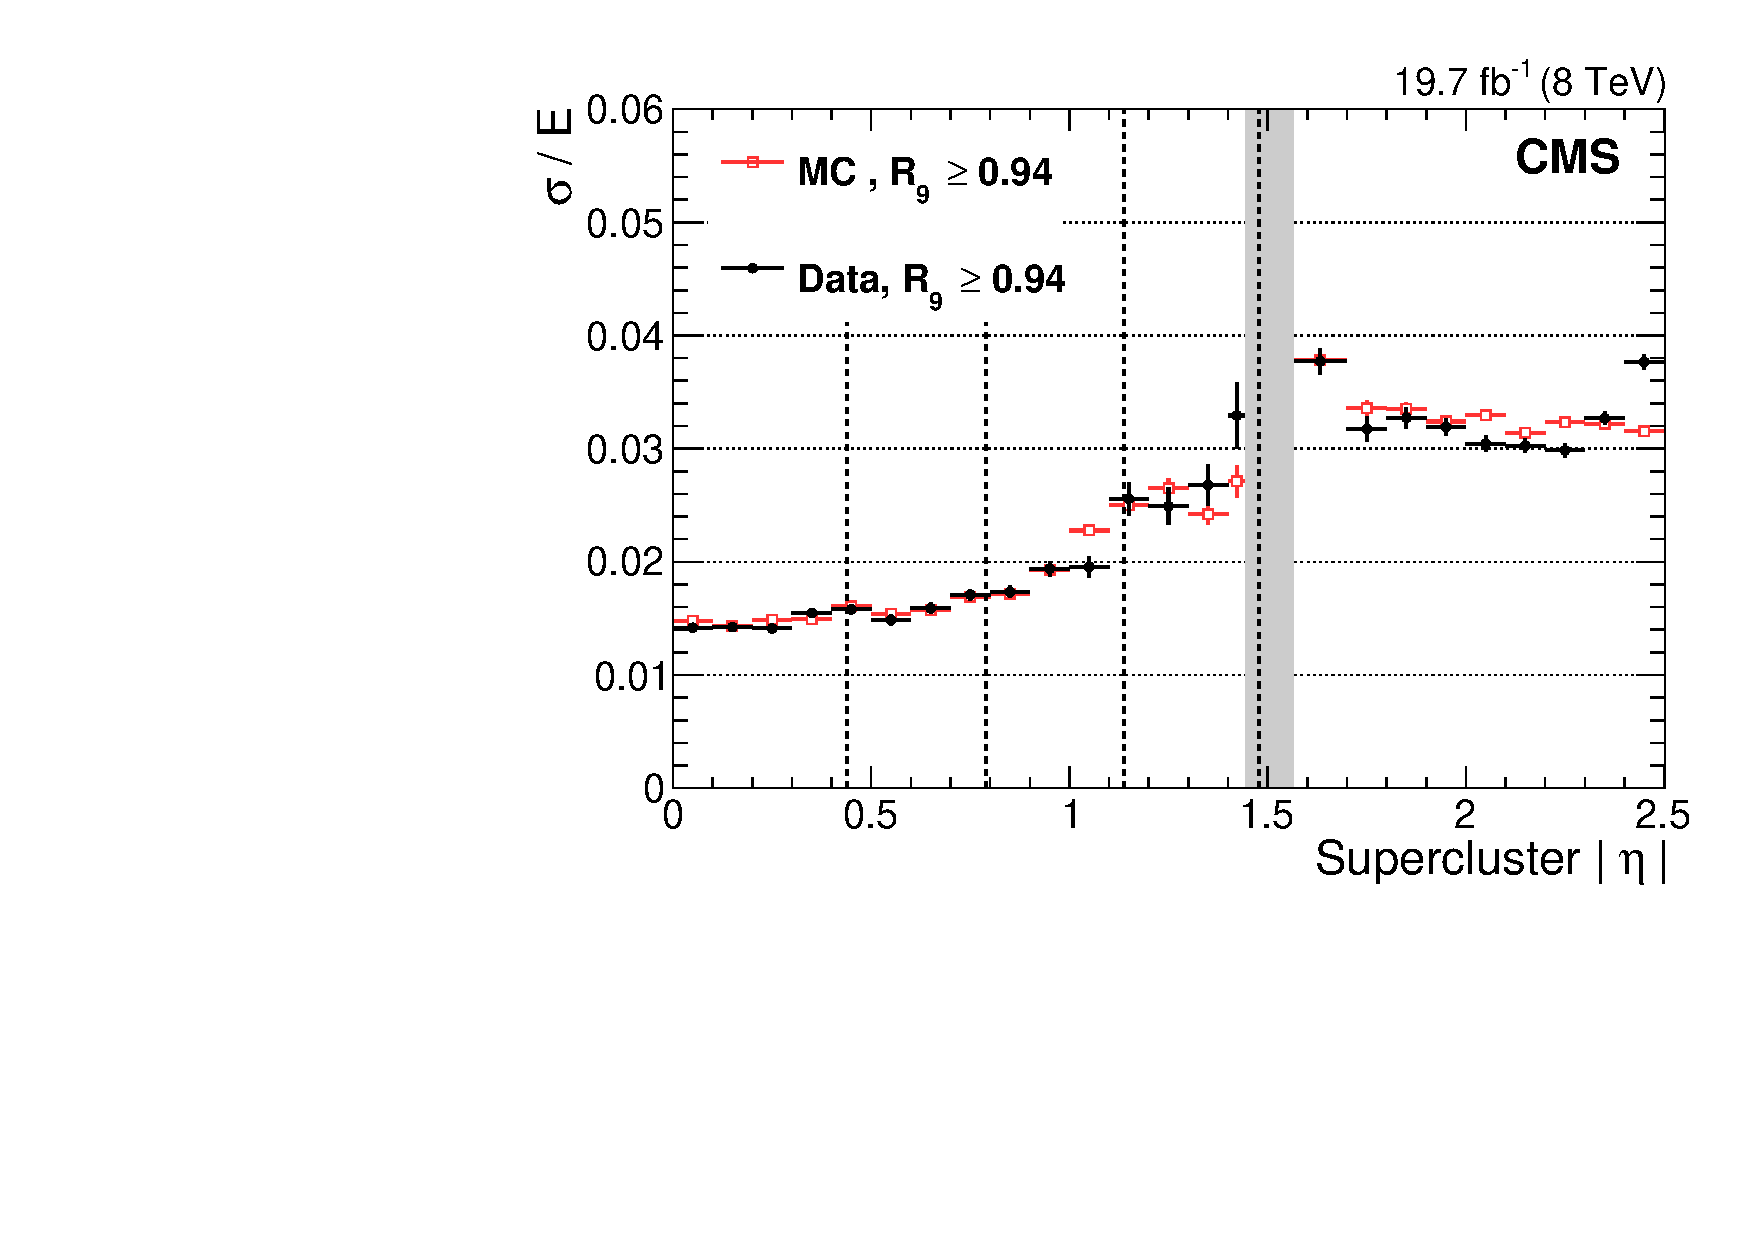
\includegraphics[width=3.0in]{resolution_highR9_aftersmear}\label{fig:energy_resol_smeared}}
    \caption{Relative electron (ECAL) energy resolution unfolded in bins of pseudo-rapidity $\vert\eta\vert$ for the barrel and the endcaps. Electrons from $Z\to ee$ decays are used. The resolution is shown for low bremsstrahlung electrons ($R_9>0.94$ with $R_9 = E_{3 \times 3} / E_{SC}$). For Fig. (a), the default simulation is used, while in Fig. (b) the tuned simulation is shown. ~\label{energy_resol}}
  \end{center}
\end{figure}
%

Several improvements to the ECAL simulation have been made from detailed comparisons with Run I data, and these will be used by default in the Run II simulations. Firstly a run-dependent simulation has been developed which mimics the evolving conditions, in terms of pileup, noise due to the radiation-induced increase of the APD dark current in the barrel (which increases the level of electronic noise) and crystal transparency losses. Figure~\ref{fig:idark} illustrates the evolution of the dark current measured for the barrel APDs operated at gain 50 and kept at 18$^\circ$C. 
%
\begin{figure}[!t]
  \begin{center}
    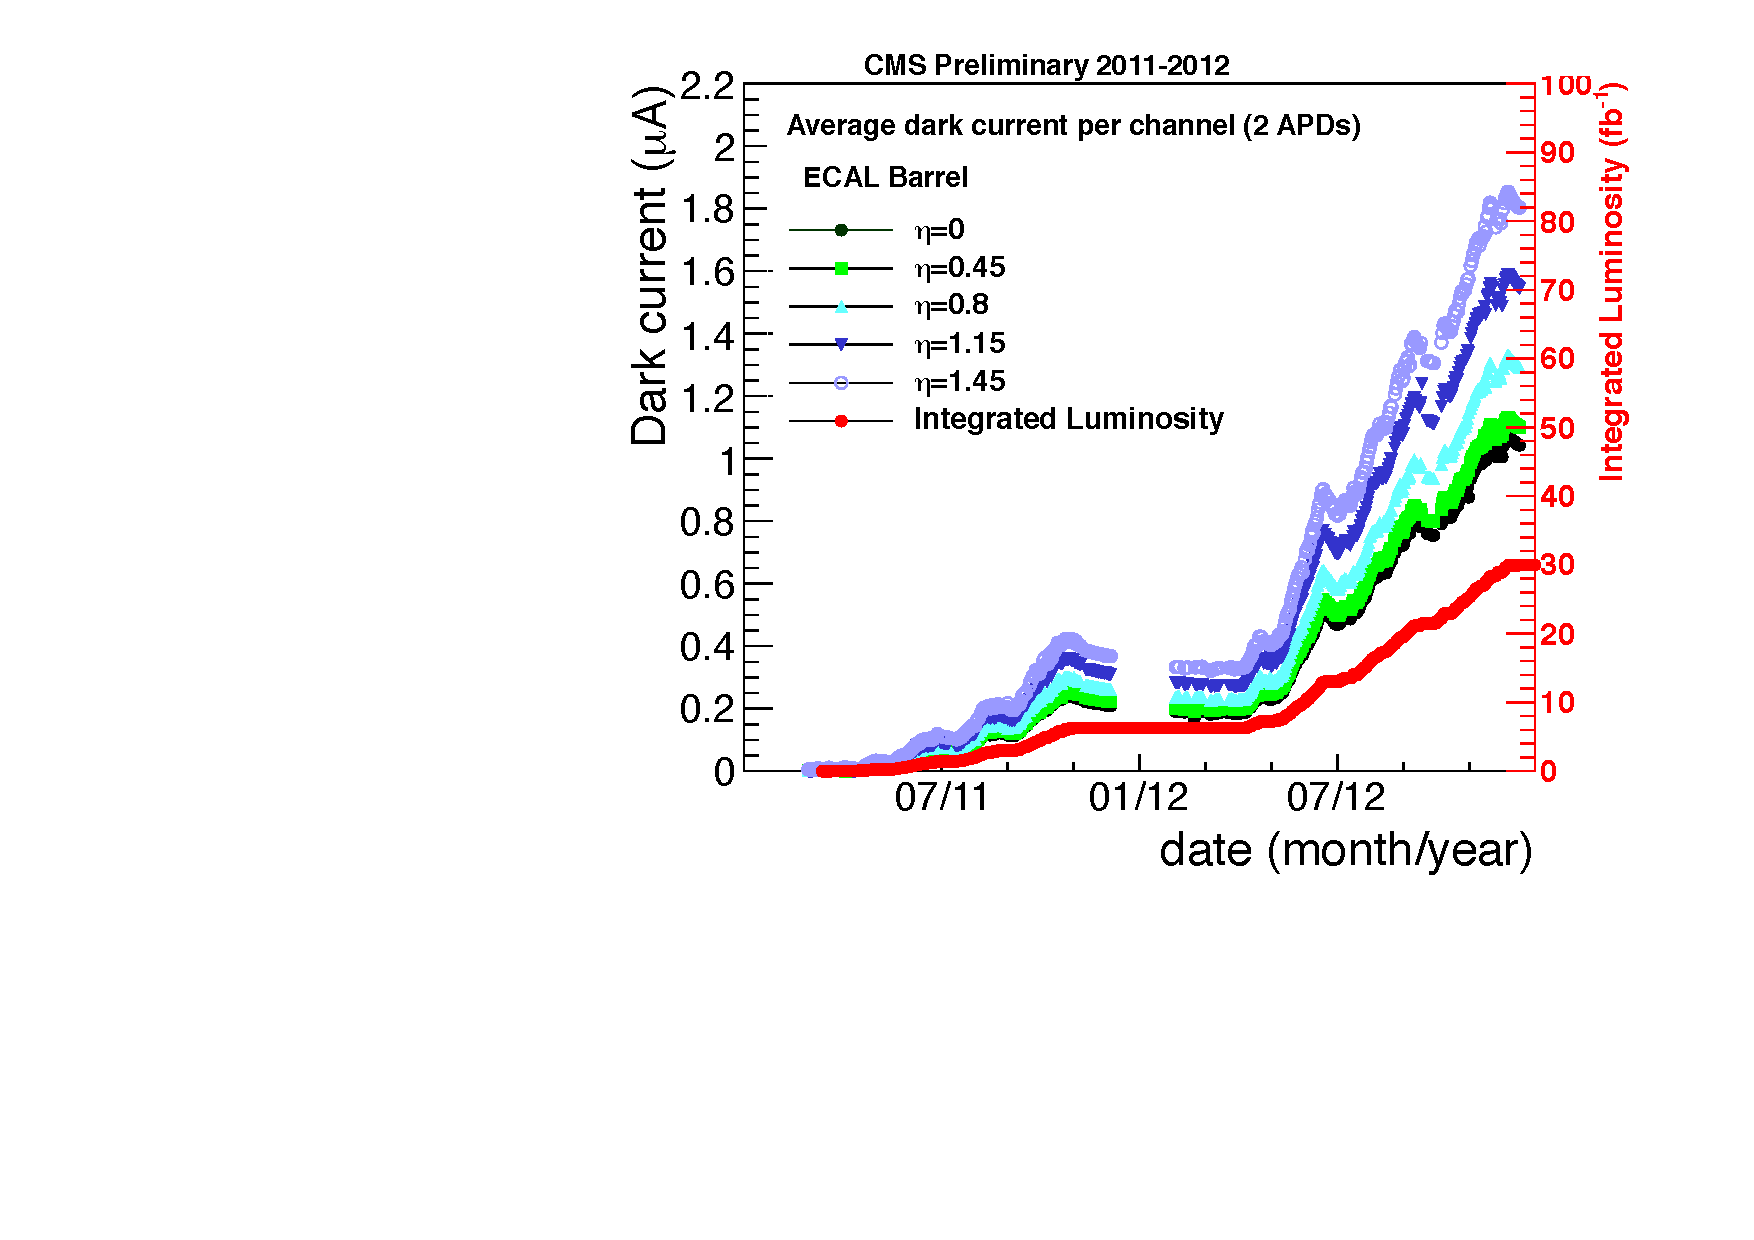
\includegraphics[width=3.3in]{HV_avg_history}
    \caption{Dark current evolution of the Avalanche Photodiodes installed in the ECAL Barrel (2 APDs are installed on each crystal). The plot shows the average dark current measured per channel as a function of time. The colors indicate different eta regions of the ECAL barrel. The delivered luminosity is also shown. \label{fig:idark}}
  \end{center}
\end{figure}
%
The run-dependent Monte Carlo (not shown in Fig.~\ref{energy_resol}) has been used to derive the results of the search of the Higgs bosons in the decay channel H$\to\gamma\gamma$~\cite{Khachatryan:2014ira}.

The amount of material between the interaction point and the ECAL affects the energy resolution for photons that convert in the tracker, and for electrons that shower. Thus to achieve a good estimate of the energy resolution an accurate description of the tracker material budget in the simulation is needed. 
With LHC Run I data it has been possible to improve the measurement of the amount of material in front of the ECAL, mostly due to the tracker. Methods using the energy loss of charged tracks, the energy loss of electrons, the comparison between collisions taken with and without magnetic field, and the ratio between the energy deposits in the preshower and the corresponding clusters in the endcaps have been developed. These data-driven methods indicate more material than predicted by MC in the region $\vert\eta\vert \sim 0.4$ and in the region $\vert\eta\vert>1$, as shown in Fig.~\ref{fig:material}. The independent methods agree, and these measurements are combined to adjust the distribution of material in the MC, in order to match the observed data.
%
\begin{figure}[!t]
  \begin{center}
    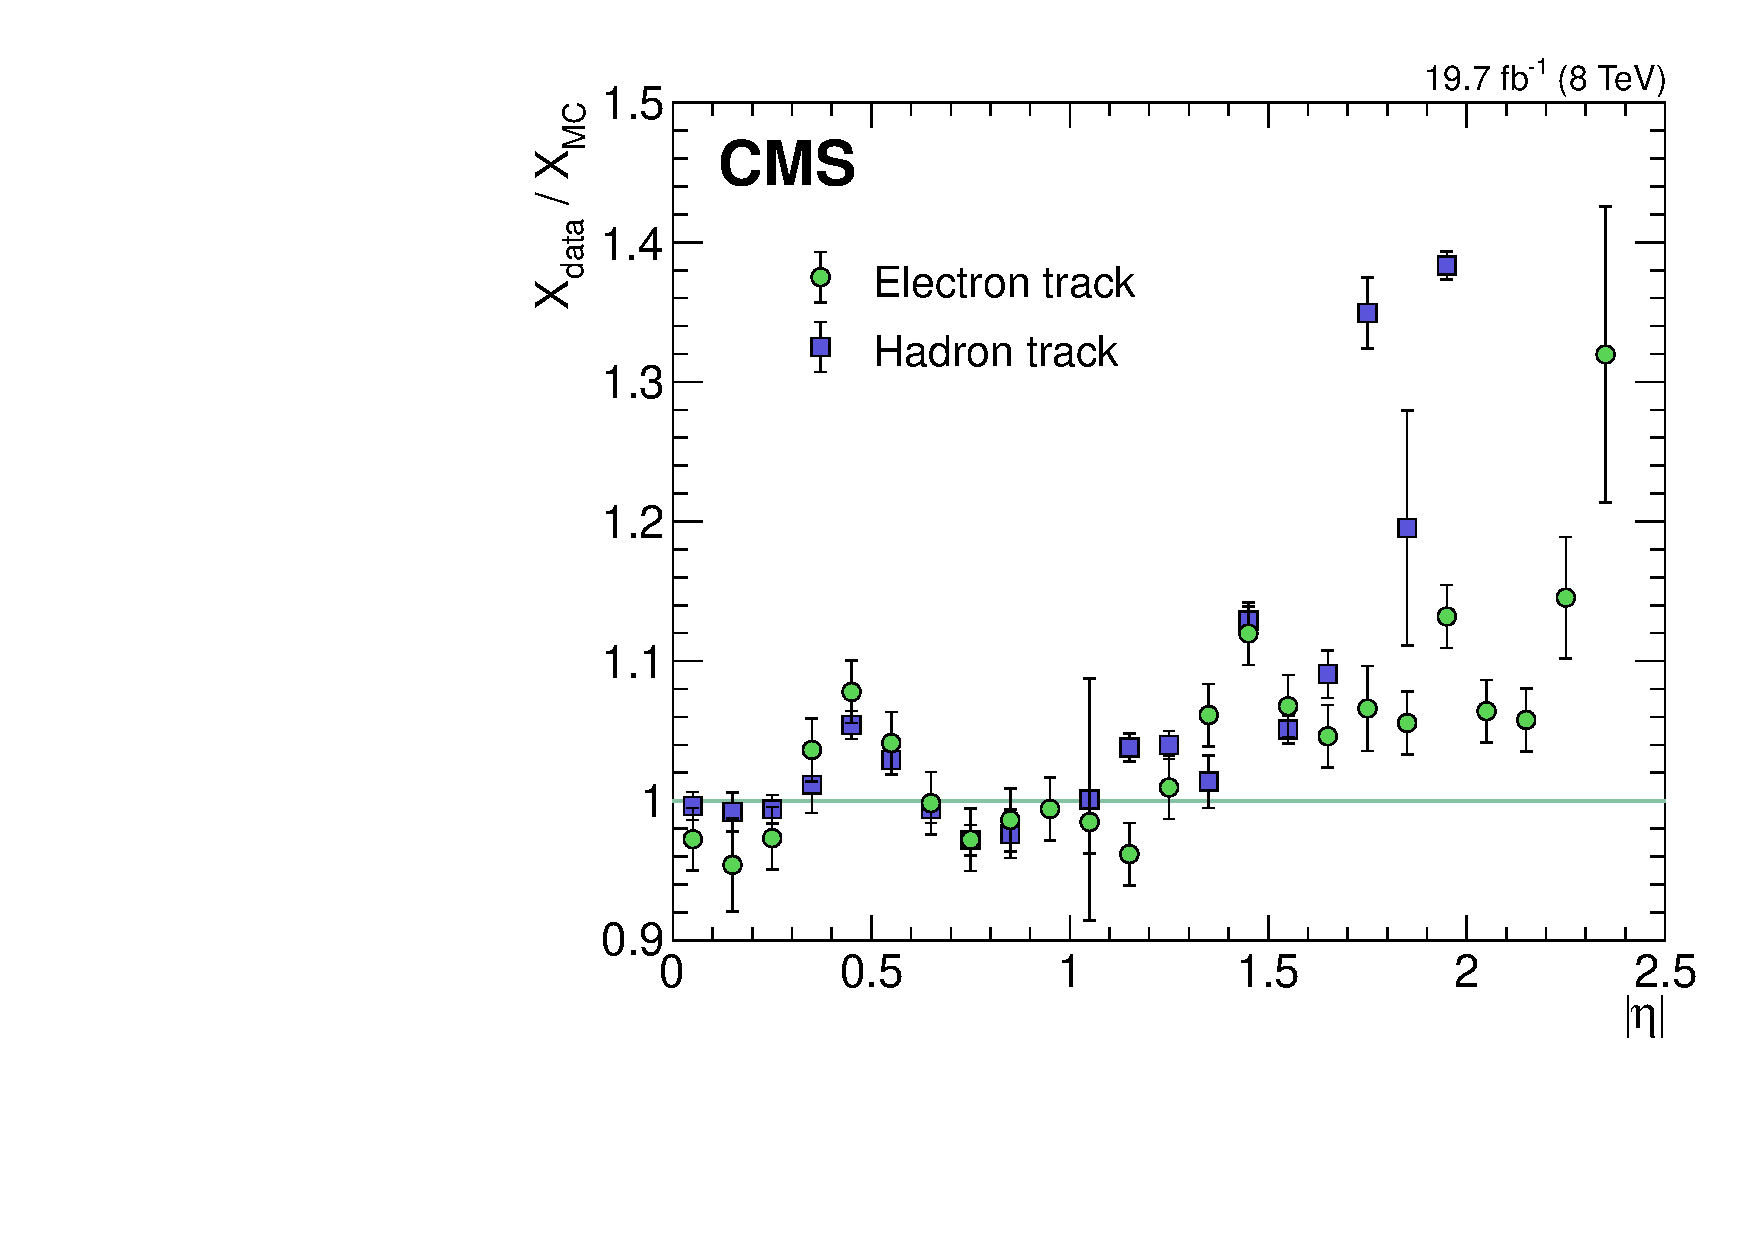
\includegraphics[width=3.0in]{material}
    \caption{Tracker material thickness (in terms of radiation lengths) estimated in the data, $X_\mathrm{data}$, relative to that estimated in simulated events, $X_\mathrm{MC}$, as a function of $\vert\eta\vert$, using electrons in $Z\to ee$ events (circles), and low momentum charged hadrons (squares). \label{fig:material}}
  \end{center}
\end{figure}
%


\section{Time reconstruction}
\label{sec:timereco}
\IEEEPARstart{T}{o} maintain an excellent energy resolution a stability of the time synchronization of the order of 1 ns is required. Moreover, a time determination with a precision better than $\sim$1 ns can be used to reject backgrounds with a broad time distribution, such as out-of-time proton-proton interactions, cosmic rays, beam halo muons. The estimate of the arrival time of a photon into ECAL can be also explicitly used to put constraints on the presence of long-lived particles predicted by models beyond the Standard Model decaying into photons which reach the ECAL out-of-time with respect to particles traveling at the speed of light from the interaction point~\cite{Chatrchyan:2012ir}. To achieve these goals the time resolution both at low energy (1 GeV or less for out-of-time particles degrading jets and $\ETslash$ resolution) and high energy (several tens of GeV for showering photons) becomes relevant.

Because of time-of-flight variations across the ECAL and different intrinsic delays among crystals, a crystal-to-crystal synchronization of the ECAL is necessary. This is achieved with a hardware procedure in the front-end electronics, that allows adjustements of groups of $5 \times 5$ groups of crystals in steps of 1.04 ns and with a software procedure, that applies a further single channel synchronization. The latter is determined by physics processes, such as minimum bias events in LHC collisions events.

The scintillation decay time of the crystals is comparable to the LHC bunch crossing interval of 25 ns (about 80\% of the light is emitted in 25 ns). The time of each ECAL hit can be measured through the ratios of the 10 consecutive digitized samples of the pulse shape. The two alternative representations of the pulse shape are shown in Fig.~\ref{fig:pulse_shapes_funcs}: the amplitude as a function of the difference between the time of the ADC sample ($T$) and the time of the maximum of the pulse ($T_{\rm max}$) and the time difference $T-T_{\rm max}$ as a function of the ratio of the amplitudes in two consecutive samples. The latter is used for the time estimate \cite{Chatrchyan:2009aj}.  
%
\begin{figure}[!t]
  \begin{center}
    \subfigure[]{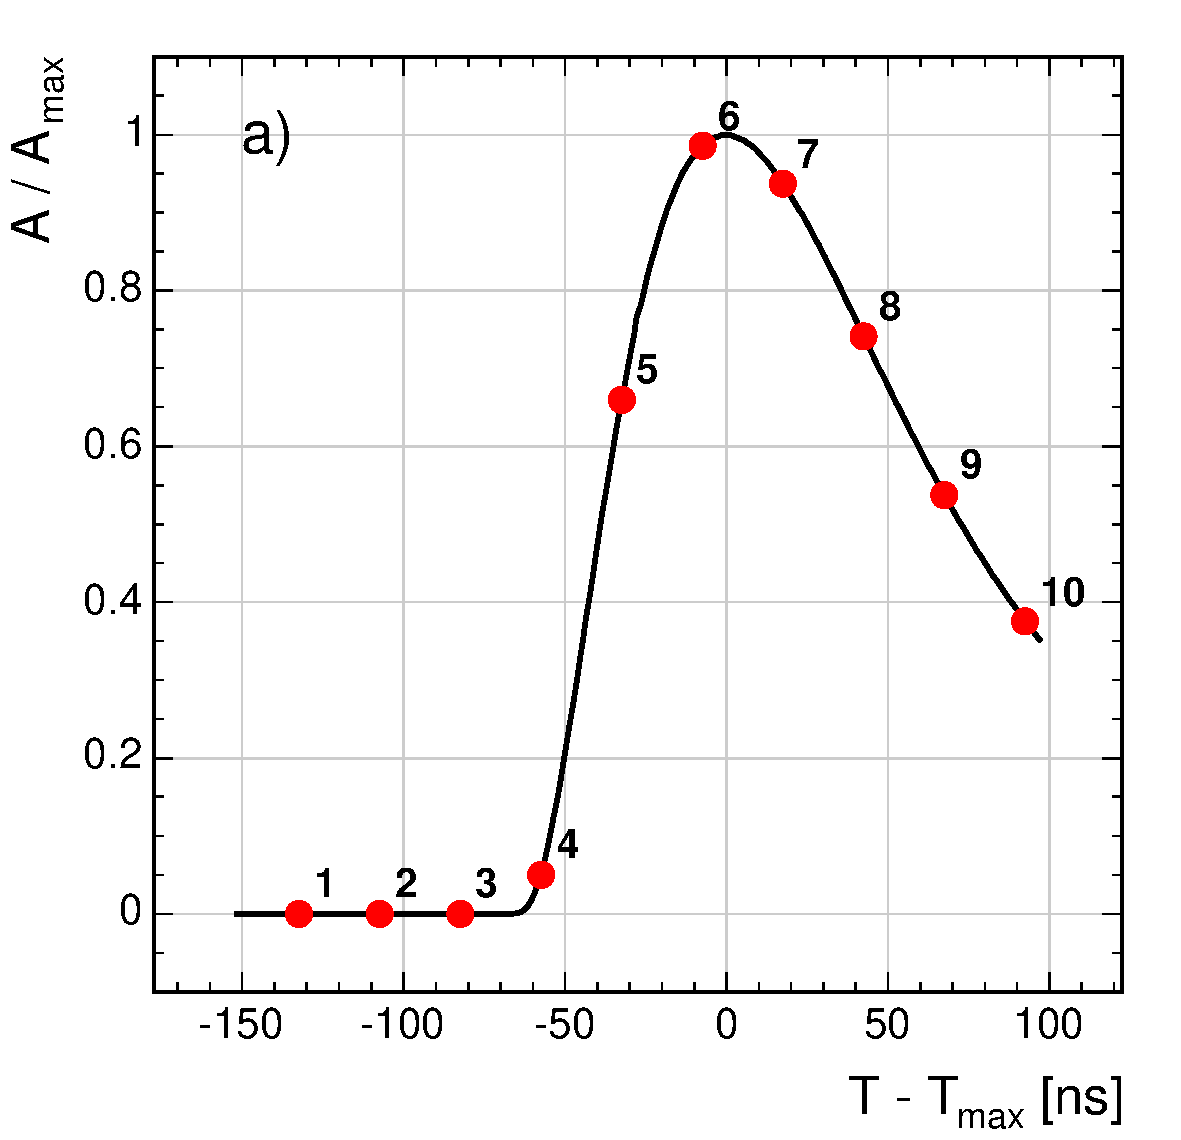
\includegraphics[width=1.7in]{pulseshape}\label{fig:pulse_shapes_normal}}
    \subfigure[]{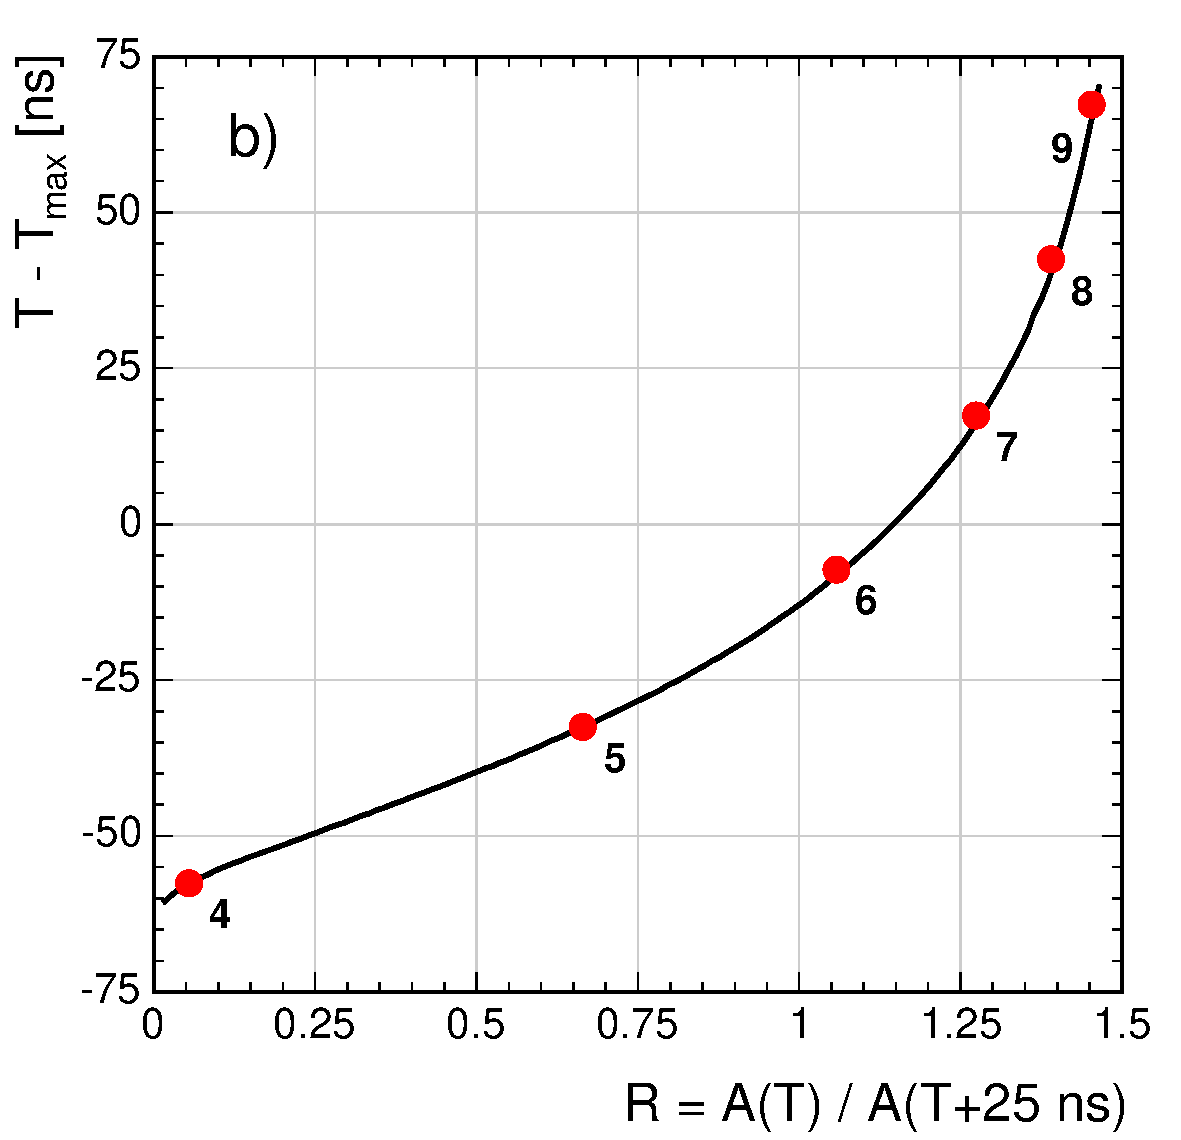
\includegraphics[width=1.7in]{ratio}\label{fig:pulse_shapes_ratio}}
    \caption{Typical ECAL pulse shape, with the 10 discrete samples shown as dots, as a function of $T-T_{\rm max}$, defined in the text (a). The pedestal has been subtracted and the samples normalized to the maximum amplitude. The solid line is the average pulse shape, as measured with a beam of electrons triggered asynchronously with respect to the digitizer clock phase. (b): Pulse shape representation using $T-T_{\rm max}$ as a function of the ratio of the amplitudes in two consecutive samples ($R$). \label{fig:pulse_shapes_funcs}}
  \end{center}
\end{figure}
%
The time reconstruction algorithm is in general degraded when more than one overlapping pulse is present.  For the high energy pulses, relevant to the beyond Standard Model signals, the low occupancy of pileup particles in the same crystal with a comparable energy will be still small in Run II, thus the same algorithm is foreseen to be used in 2015.


\section{Time resolution measurement}
\label{sec:timeresolution}
\IEEEPARstart{T}{he} time resolution is extracted by comparing the time measured in ECAL hits that are synchronous. Two methods are used to measure it using collision data.

The first method compares the time of the two electrons from $Z\to e^+e^-$ decays. The time is corrected by the time-of-flight of the electrons from the primary vertex position, obtained from the electron tracks. The two SCs are required to have an electromagnetic-like cluster shape, and the resulting invariant mass must be consistent with the Z boson mass. The energy of both seeds must fulfill 10 GeV $<E<$ 120 GeV. The resolution is extracted as the $\sigma$ parameter of a Gaussian fit to the core of the time difference between the two seeds. Figure \ref{fig:time_resol_zee} shows the resulting resolution plotted as a function of the effective amplitude $A_{\rm eff} = A_1 A_2 \sqrt{A_1^2 + A_2^2}$, where $A_1$ and $A_2$ are the amplitudes of the two SC seeds. The noise term, $N$ is very similar to that obtained in electron beam test and the constant term, $C$ is estimated be $\approx$ 150 ps. This value is much better then the one needed to achieve the best energy resolution (1 ns), and allows the searches of signatures from BSM particles, e.g. those in Ref.~\cite{Chatrchyan:2012ir}. 

The second method compares the two most energetic neighboring crystals of a photon cluster. Additional selection criteria are applied, based on the shape of the ECAL cluster and on the energy of the ECAL hit (E $<$ 120 GeV). The resulting resolution, plotted as a function of the effective amplitude, shows a smaller constant term than that measured with $Z\to e^+e^-$ decays, of about 70 ps, shown in Fig.~\ref{fig:time_resol_neighbors}. This result is closer to the test beam results.

While these excellent values of the time determination resolution, measured during LHC collisions are beyond the needs for the target energy resolution, and were successfully used in physics analyses, they are larger than the intrinsic resolution of the ECAL measured in ideal conditions (no magnetic field, no irradiation, no material in front of the crystals) during the test beam ($\sim$ 20 ps) \cite{Chatrchyan:2009aj}. It is therefore of interest to investigate this further, both to optimise the timing measurements in CMS and to understand the fundamental limitations in resolution for future detectors that use precision timing (better than $\sim$ 10 ps) for out-of-time pileup mitigation. A study has been performed, comparing crystals belonging to either the same or different readout units. The readout unit corresponds to a trigger tower which is a $5 \times 5$ matrix of crystals.  The different constant term obtained in the two cases, 67 ps vs 130 ps, does not explain the difference with respect to the test beam results but indicates that there are systematic effects related to the clock distribution to the individual readout units, rather than a residual timing jitter. This hypothesis will be further investigated with future studies using Run II data.
%
\begin{figure}[!t]
  \begin{center}
    \subfigure[]{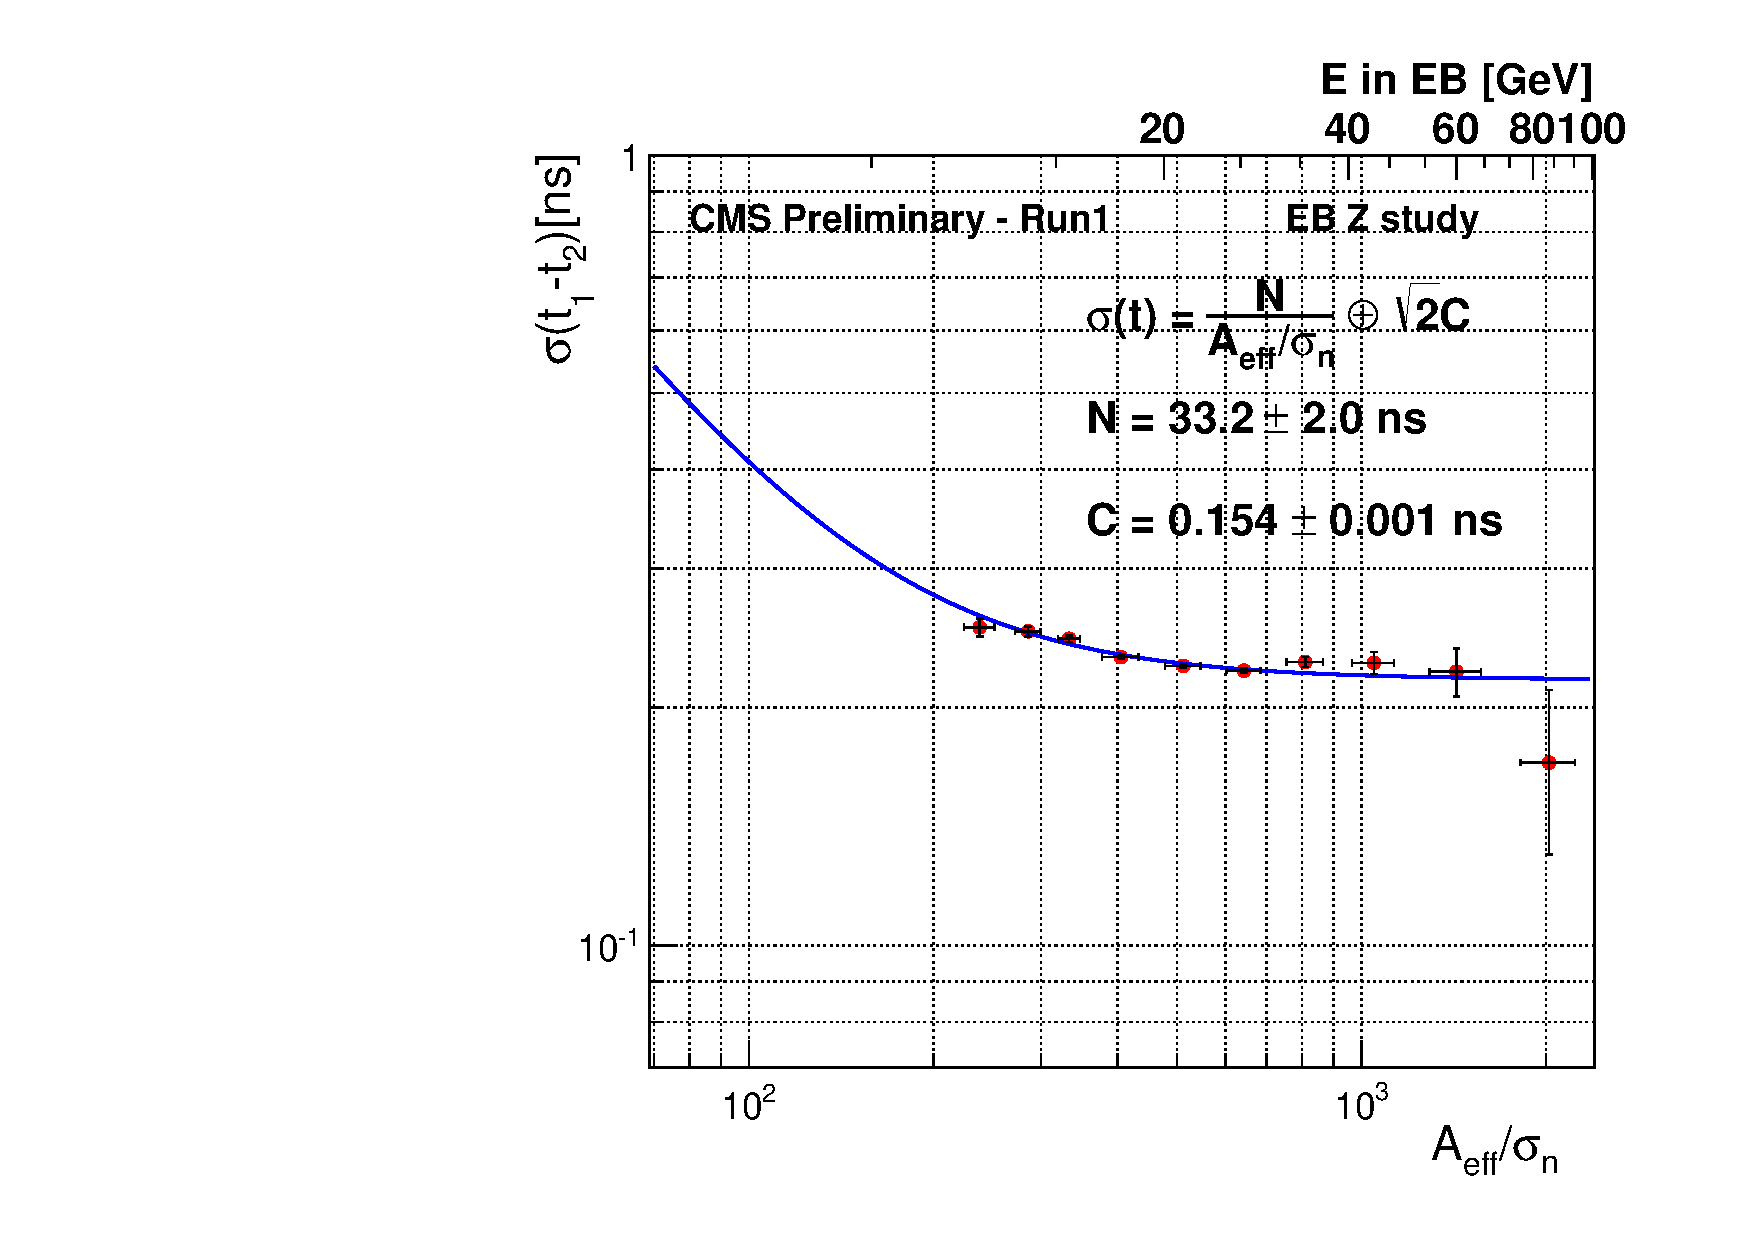
\includegraphics[width=3.0in]{time_resol_Z}\label{fig:time_resol_zee}}
    \subfigure[]{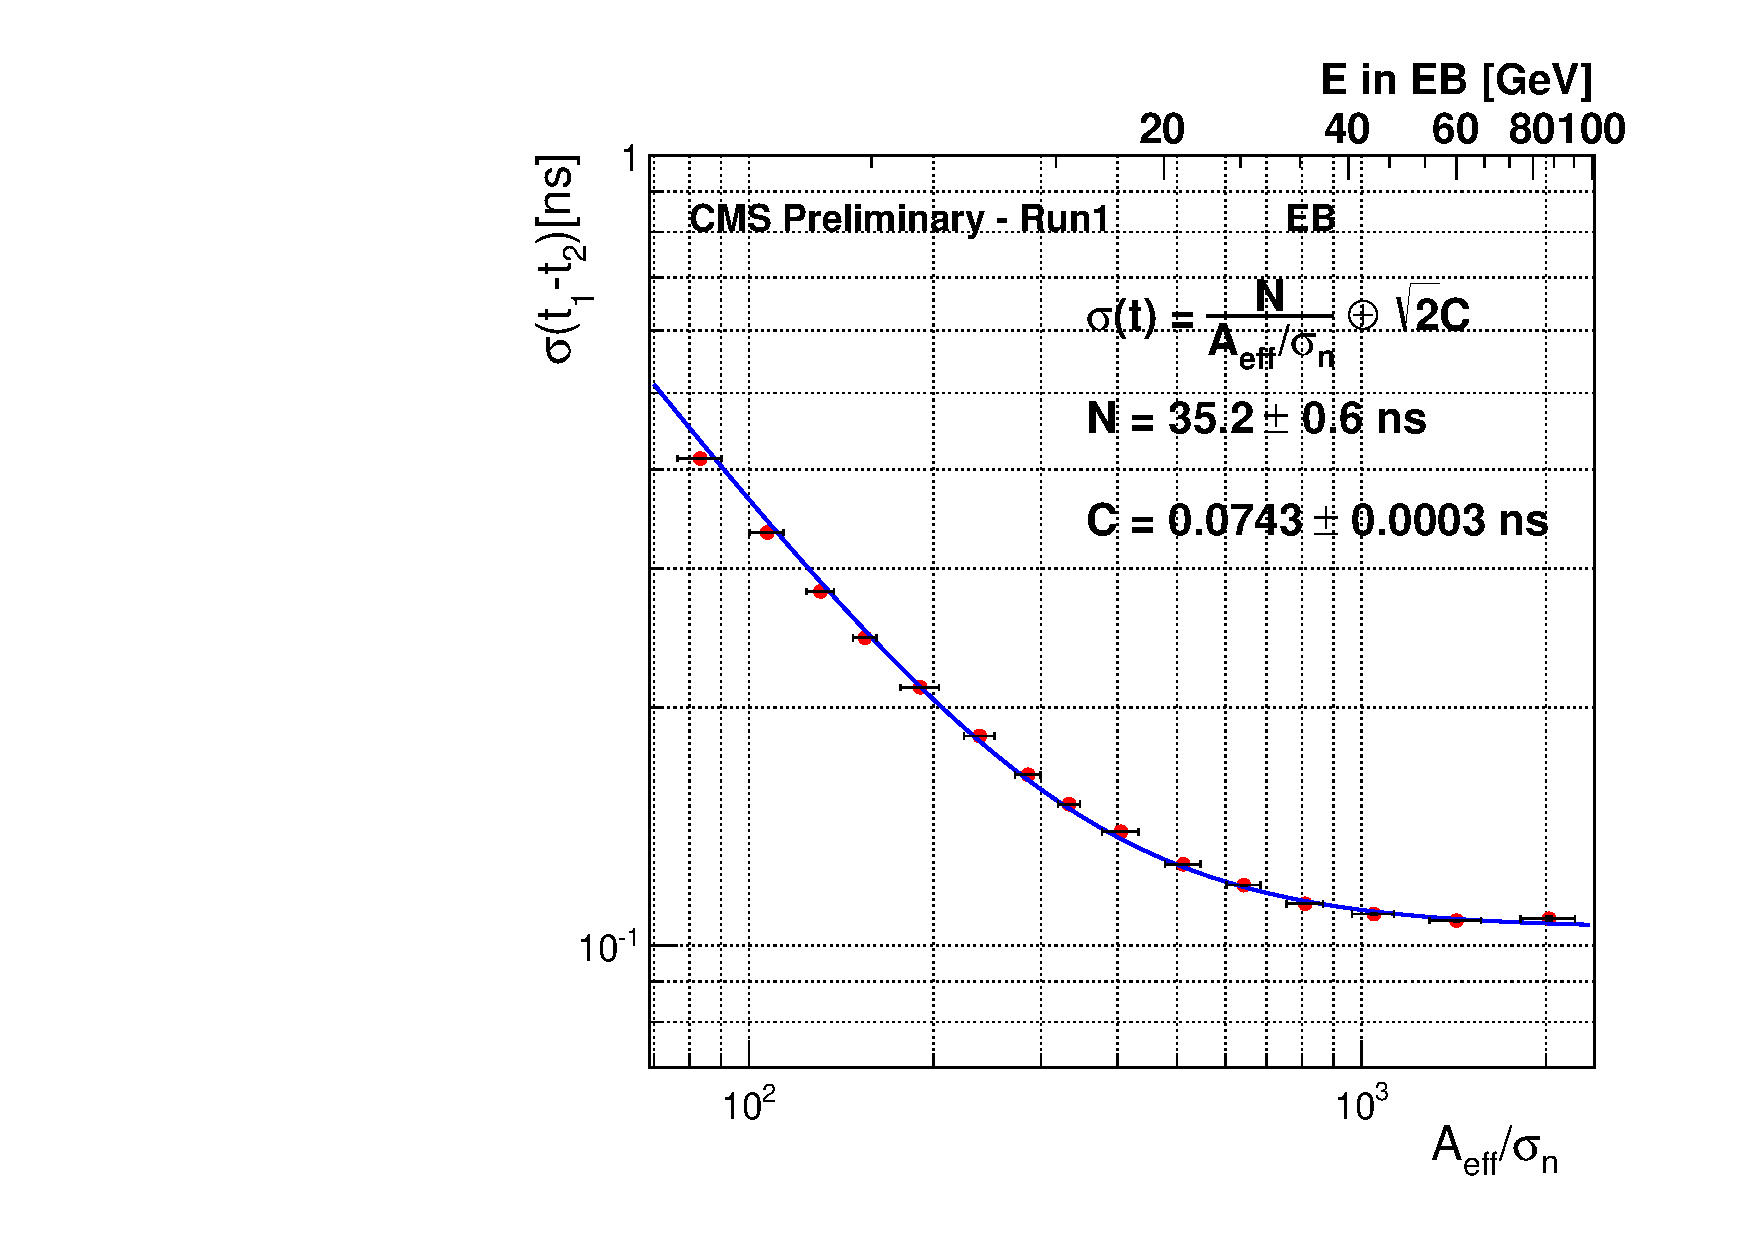
\includegraphics[width=3.0in]{time_resol_neighbors}\label{fig:time_resol_neighbors}}
    \caption{Resolution measured from the time difference between the two electrons from $Z\to ee$ decays, as a function of the effective amplitude $A_{\rm eff}$ defined in the text, normalized to the noise in the ECAL Barrel for Run I data (a). Resolution of the time difference between the two most energetic crystals of an ECAL cluster as a function of $A_{\rm eff}$ (b). \label{fig:time_resol}}
  \end{center}
\end{figure}
%



\section{Conclusion}
\label{sec:conclusions}
The electromagnetic calorimeter of CMS has demonstrated excellent performance during LHC Run I, and it has been essential in the search for the Higgs boson and in the determination of its properties. The excellent timing performance of the calorimeter has also enabled CMS to extend the reach for physics beyond the Standard Model. The harsh environment of the LHC has required a continuous effort in the operation, monitoring and calibration, and simulation of the calorimeter. 

For the forthcoming Run II at $\sqrt{s}=13$ TeV with an increased instantaneous luminosity, an almost doubled number of pileup interactions and the reduced bunch spacing from 50 ns to 25 ns will make the environment even harsher. A new ECAL amplitude reconstruction have been developed and tested, showing that the contribution of the out-of-time pileup energy can be reduced to a negligible level. The optimised calibration procedures and techniques will be maintained and will serve as the basis for the next data taking period, with a re-optimization of the streams, which has been performed during the shutdown period between Run I and Run II. These improvements will allow ECAL to maintain excellent performance during LHC Run II, both for precision physics including Higgs boson properties and other SM measurements, and for the searches of BSM particles with decay chains involving electrons and photons.


% Can use something like this to put references on a page
% by themselves when using endfloat and the captionsoff option.
\ifCLASSOPTIONcaptionsoff
  \newpage
\fi


\begin{thebibliography}{1}

\bibitem{Chatrchyan:2008aa} 
  S.~Chatrchyan {\it et al.}  [CMS Collaboration], ``The CMS experiment at the CERN LHC,'' JINST {\bf 3}, S08004 (2008).

\bibitem{CMS:1997ema} 
  [CMS Collaboration], ``CMS: The electromagnetic calorimeter. Technical design report,''  CERN-LHCC-97-33, CMS-TDR-4.

\bibitem{Khachatryan:2014ira} 
  V.~Khachatryan {\it et al.}  [CMS Collaboration], ``Observation of the diphoton decay of the Higgs boson and measurement of its properties,''  Eur.\ Phys.\ J.\ C {\bf 74}, no. 10, 3076 (2014)

\bibitem{Chatrchyan:2013mxa} 
  S.~Chatrchyan {\it et al.}  [CMS Collaboration], ``Measurement of the properties of a Higgs boson in the four-lepton final state,''
  Phys.\ Rev.\ D {\bf 89}, 092007 (2014)

\bibitem{Raymond:2005jm} 
  M.~Raymond, G.~Hall, J.~Crooks and M.~French, ``The MGPA electromagnetic calorimeter readout chip for CMS,''
  IEEE Trans.\ Nucl.\ Sci.\  {\bf 52}, 756 (2005).

\bibitem{nnls}
J.~Cantarella and M.~Piatek, ``Tsnnls: A solver for large sparse least squares problems with non-negative variables,'' CoRR-cs.MS/0408029 (2004)

\bibitem{Bruneliere:2006ra} 
  P.~Adzic {\it et al.}, ``Reconstruction of the signal amplitude of the CMS electromagnetic calorimeter,''  Eur.\ Phys.\ J.\ C {\bf 46S1}, 23 (2006).

\bibitem{Chatrchyan:2013dga} 
  S.~Chatrchyan {\it et al.}  [CMS Collaboration], ``Energy Calibration and Resolution of the CMS Electromagnetic Calorimeter in $pp$ Collisions at $\sqrt{s} = 7$ TeV,''   JINST {\bf 8}, P09009 (2013)

\bibitem{Anfreville:2007zz} 
  M.~Anfreville {\it et al.}, ``Laser monitoring system for the CMS lead tungstate crystal calorimeter,''  Nucl.\ Instrum.\ Meth.\ A {\bf 594}, 292 (2008).

\bibitem{CMS:2010eua} 
  [CMS Collaboration], ``Commissioning of the Particle-Flow reconstruction in Minimum-Bias and Jet Events from pp Collisions at 7 TeV,''  CMS-PAS-PFT-10-002.

\bibitem{Chatrchyan:2012ir} 
  S.~Chatrchyan {\it et al.}  [CMS Collaboration], ``Search for new physics with long-lived particles decaying to photons and missing energy in $pp$ collisions at $\sqrt{s}=7$ TeV,''  JHEP {\bf 1211}, 172 (2012)

\bibitem{Chatrchyan:2009aj} 
  S.~Chatrchyan {\it et al.}  [CMS Collaboration], ``Time Reconstruction and Performance of the CMS Electromagnetic Calorimeter,''  JINST {\bf 5}, T03011 (2010)

\bibitem{Gadomski:1992xu} 
  S.~Gadomski, G.~Hall, T.~Hogh, P.~Jalocha, E.~Nygard and P.~Weilhammer, ``The Deconvolution method of fast pulse shaping at hadron colliders,''  Nucl.\ Instrum.\ Meth.\ A {\bf 320}, 217 (1992).

\end{thebibliography}


% that's all folks
\end{document}


